
% Monografia TCC - Projeto Vindex
% Template politex para Escola Politécnica da USP
\documentclass[]{politex}

% Idioma principal: português brasileiro
\usepackage[brazil]{babel}
% Pacote para URLs
\usepackage{url}
% Pacotes gráficos e utilitários
\usepackage{graphicx}
\usepackage{caption}
\usepackage{booktabs}
\usepackage{listings}
\usepackage{xcolor}
% Pacote de matemática que define \text e outros comandos em ambiente matemático
\usepackage{amsmath}
\usepackage{tikz}
\usetikzlibrary{arrows,positioning}

% Configurações para o pacote listings (códigos-fonte)
\renewcommand{\lstlistingname}{Listagem}
\renewcommand{\lstlistlistingname}{Lista de Listagens}
% Configuração padrão do ambiente de listagens. Note que a vírgula após a
% linguagem evita que o comentário interfira na definição.
\lstset{
  basicstyle=\footnotesize\ttfamily,
  breaklines=true,
  keywordstyle=\bfseries\color{blue!70},
  commentstyle=\itshape\color{green!50!black},
  stringstyle=\color{orange},
  numbers=left,
  numberstyle=\tiny,
  numbersep=5pt,
  language=C++, % (pode ser ajustado por listagem individual)
}

% Informações de dados para CAPA e FOLHA DE ROSTO
\titulo{Sistema de
Detecção de Acidentes e Alerta Automático para Motociclistas}
% Define os autores conforme o template politeX
\autor{Igor Teixeira Lacerda \\ Lorenzo Bighetti Zauith \\ Rodrigo Costa de Araújo}
\local{São Paulo}
\data{2025}

% Tipo de documento: TCC
\tcc{Engenheiro Eletricista}

% Departamento e área
\departamento{Engenharia Elétrica}
\areaConcentracao{Eletrônica e Sistemas Computacionais}

% Orientador
\orientador{Márcio Lobo Netto}

\begin{document}
% ========== Capa e folhas de rosto ==========
\capa
\falsafolhaderosto
\folhaderosto


% ========== Dedicatória (opcional) ==========
\dedicatoria{Dedicamos este trabalho a todos os motociclistas que inspiraram esta pesquisa e às nossas famílias pelo apoio incondicional durante todo o desenvolvimento deste projeto.}


% ========== Resumo ==========
\begin{resumo}
Os acidentes motociclísticos representam uma das principais causas de mortalidade no trânsito brasileiro. Segundo a Associação Brasileira de Medicina do Tráfego (ABRAMET), a cada 39 minutos um motociclista perde a vida no trânsito
brasileiro\cite{czerwonka2025}, e a taxa de mortalidade por quilômetro
rodado é cerca de 30~vezes maior do que a de ocupantes de automóveis. A
vulnerabilidade desses condutores agrava-se quando o acidente ocorre em
vias de baixa circulação, áreas rurais ou estradas com pouca iluminação
e monitoramento. Nesses cenários, o tempo até que alguém identifique o
acidente e acione o resgate pode ultrapassar a chamada “hora de ouro”,
intervalo de até 60 minutos após um trauma grave, considerado crítico
para a sobrevivência \cite{tsaco2020}. Estudos demonstram que vítimas de acidentes graves têm até
60\% mais chances de sobreviver quando socorridas nos primeiros 30
minutos \cite{champion2016}. Diante desse quadro, este trabalho propõe o
desenvolvimento de um sistema embarcado de baixo custo, fixado na
estrutura da motocicleta, capaz de detectar automaticamente acidentes
por meio de sensores inerciais, enviar alertas de emergência com
localização geográfica em tempo real e, adicionalmente, registrar
imagens do momento da colisão como apoio secundário para diagnóstico ou
documentação do ocorrido. O dispositivo é composto por um
microcontrolador Placa Computacional, um microcontrolador Node MCU
Super Mini, um sensor GY-BMI160 (acelerômetro e giroscópio) e uma câmera
grande angular de 160°, integrados em uma carcaça impressa em 3D
projetada para resistir a impactos. A lógica de funcionamento baseia-se
na análise de padrões de aceleração e variação angular para detectar
quedas abruptas ou mudanças anormais de orientação, desencadeando
automaticamente o protocolo de emergência sem necessidade de intervenção
do usuário. A transmissão dos dados é feita via conexão Bluetooth,
enviando as coordenadas do acidente e uma mensagem pré-configurada para
contatos de emergência ou serviços especializados. A câmera, posicionada
com ângulo amplo, atua como ferramenta auxiliar e pode registrar imagens
de forma instantânea após o acidente, gerando evidência visual útil. O
sistema é alimentado por bateria recarregável com autonomia de
aproximadamente 10 horas de monitoramento contínuo. Com custo estimado
em R\$~300,00 por unidade, o projeto visa tornar acessível uma
tecnologia crítica para mitigar o impacto de acidentes motociclísticos,
com potencial de aplicação em escala nacional por órgãos públicos,
seguradoras e fabricantes. Além de seu caráter social, a proposta
alinha-se às tendências de segurança ativa e resposta emergencial em
tempo real, reforçando o papel da engenharia embarcada na preservação da
vida.

\textbf{Palavras-Chave}: segurança veicular; acidentes de moto; sistemas
embarcados; detecção automática; resposta emergencial.
\end{resumo}


% ========== Abstract ==========
\begin{abstract}
Motorcycle accidents are a
leading cause of traffic fatalities in Brazil. According to the
Brazilian Association of Traffic Medicine (ABRAMET), a motorcyclist dies
every 39 minutes in Brazil, and the fatality rate per kilometer traveled
is dozens of times higher than that of car
occupants\cite{czerwonka2025}. The vulnerability of these riders is
exacerbated when accidents occur on low-traffic roads, rural areas, or
poorly lit and monitored highways. In such situations, the time until an
accident is identified and rescue is activated can exceed the “golden
hour,” a critical 60-minute window after severe trauma, vital for
survival. Studies demonstrate that severe accident victims have up to a 60\% higher
chance of survival when rescued within the first 30
minutes \cite{champion2016}. Given this scenario, this work proposes the
development of a low-cost embedded system, mounted on the motorcycle’s
frame, capable of automatically detecting accidents using inertial
sensors, sending real-time emergency alerts with geographical location,
and additionally recording images of the collision moment as secondary
support for diagnosis or documentation. The device comprises a Placa Computacional microcontroller, an Node MCU Super Mini microcontroller, a
GY-BMI160 sensor (accelerometer and gyroscope), and a 160-degree
wide-angle camera, all integrated into a 3D-printed enclosure designed
to withstand impact. The system’s operational logic is based on
analyzing acceleration patterns and angular variations to detect abrupt
falls or abnormal orientation changes, automatically triggering the
emergency protocol without user intervention. Data transmission occurs
via Bluetooth connection, sending accident coordinates and a
pre-configured message to emergency contacts or specialized services.
The wide-angle camera acts as an auxiliary tool, instantly capturing
images during and after the accident, generating useful visual evidence.
The system is powered by a rechargeable battery, providing approximately
10 hours of continuous monitoring. With an estimated cost of R\$~300.00
per unit, this project aims to make critical technology accessible to
mitigate the impact of motorcycle accidents, with potential for national
application by public agencies, insurance companies, and manufacturers.
Beyond its social impact, the proposal aligns with trends in active
safety and real-time emergency response, reinforcing the role of
embedded engineering in preserving lives.

\textbf{Keywords}: vehicle safety; motorcycle accidents; embedded
systems; automatic crash detection; emergency response.
\end{abstract}


% ========== Listas (opcional) ==========
\listadefiguras
\listadetabelas

% ========== Sumário ==========
\sumario

% ========== Listas definidas pelo usuário (opcional) ==========
\begin{pretextualsection}{Lista de Siglas}
\begin{description}
  \item[ABRAMET] Associação Brasileira de Medicina do Tráfego
  \item[BLE] \textit{Bluetooth Low Energy}
  \item[CPU] \textit{Central Processing Unit} (Unidade Central de Processamento)
  \item[Node MCU] Família de microcontroladores Node MCU (RISC-V 160~MHz com Bluetooth 5.0)
  \item[GPS] \textit{Global Positioning System} (Sistema de Posicionamento Global)
  \item[IMU] \textit{Inertial Measurement Unit} (Unidade de Medição Inercial)
  \item[NHTSA] \textit{National Highway Traffic Safety Administration}
  \item[OCR] \textit{Optical Character Recognition} (Reconhecimento Óptico de Caracteres)
  \item[RF] Requisito Funcional
  \item[RNF] Requisito Não Funcional
  \item[YOLO] \textit{You Only Look Once} (Algoritmo de detecção de objetos em tempo real)
\end{description}
\end{pretextualsection}

% Lista de símbolos
\begin{pretextualsection}{Lista de Símbolos}
\begin{description}
  \item[$g$] Aceleração gravitacional padrão ($\approx 9{,}81~\text{m/s}^2$).
  \item[$\omega$] Velocidade angular (em radianos ou graus por segundo).
  \item[$\Delta$] Variação de uma grandeza (diferença entre dois instantes ou estados).
\end{description}
\end{pretextualsection}

% Introdução
\chapter{Introdução}\label{cap:introducao}

\section{Antecedentes} A segurança no trânsito é um desafio crítico nas
grandes cidades e rodovias. No contexto de transporte individual, os
motociclistas se destacam pela alta exposição a riscos de acidentes
graves. Nas últimas décadas, avanços em sistemas eletrônicos veiculares
têm reduzido a mortalidade entre ocupantes de automóveis (por meio de
airbags, freios ABS, etc.), porém motocicletas ainda carecem de
dispositivos equivalentes de proteção ativa e de sistemas automáticos de
alerta pós-acidente. Tecnologias de chamada de emergência automática,
como o sistema \textit{eCall} implementado em carros na União Europeia,
comprovam que a rápida notificação de acidentes pode salvar vidas,
diminuindo o tempo de resposta de equipes de resgate\cite{bosch2020}.
Entretanto, tais soluções ainda não são amplamente disponíveis para
motocicletas.

Historicamente, a resposta a acidentes motociclísticos depende quase
exclusivamente de terceiros presenciarem o evento e acionar socorro. Em
áreas remotas ou horários de baixo movimento, um motociclista acidentado
pode ficar longos períodos sem assistência. Esse atraso no atendimento
médico reduz drasticamente as chances de sobrevivência, conforme
destacam estatísticas da ABRAMET \cite{abramet2025} e estudos internacionais \cite{who2018}. Pesquisas de Park \textit{et al.} \cite{park2020} demonstram a relação direta entre tempo pré-hospitalar e desfechos em trauma, enquanto Brown \textit{et al.} \cite{brown2016} evidenciam que, em casos de hemorragia, cada minuto adicional de atraso está associado a aumento significativo na mortalidade.
Esse problema motivou pesquisas em sistemas de detecção automática de
acidentes utilizando sensores inerciais, dispositivos móveis e técnicas
de telecomunicação para envio de alertas.

Com o advento de sensores MEMS (\textit{Micro-Electro-Mechanical
Systems}) acessíveis e microcontroladores de baixo custo e baixo
consumo, tornou-se viável a construção de dispositivos embarcados
capazes de monitorar continuamente o movimento de um veículo e
identificar padrões indicativos de colisão ou queda. Diversos trabalhos
exploraram o uso de acelerômetros e giroscópios para esse
fim\cite{white2011, gouvea2018}. Em paralelo, a difusão de smartphones
com sensores embutidos levou ao surgimento de aplicativos de detecção de
acidentes, embora com limitações como a dependência de o
smartphone estar fixo no veículo e ligado no momento do acidente. Nesse
contexto, um dispositivo dedicado ao veículo, integrado ao motociclo,
pode oferecer maior confiabilidade e autonomia na detecção de acidentes.

\section{Motivação} A motivação principal deste projeto é reduzir o
tempo entre a ocorrência de um acidente de moto e o atendimento à
vítima. Conforme mencionado, a ``hora de ouro'' é crucial para aumentar
a probabilidade de sobrevivência em traumas graves. No Brasil, onde
milhares de motociclistas transitam diariamente em condições adversas,
um sistema capaz de automaticamente perceber um acidente e alertar
equipes de emergência ou contatos de confiança pode significar a
diferença entre a vida e a morte em muitos casos.

Além do aspecto vital, há também motivação social e econômica. Acidentes
de moto representam custos elevados ao sistema de saúde e à seguridade
com licenças médicas, indenizações e outros gastos, e mitigá-los ou minimizar suas
consequências traz benefícios coletivos. Segundo dados da Agência Brasil \cite{agenciabrasil2025}, a frota brasileira de motocicletas cresceu 42\% entre 2015 e 2024, alcançando 35 milhões de unidades, enquanto as mortes de motociclistas correspondem a 38,6\% dos óbitos no trânsito. Tecnologias de segurança ativa
para motocicletas estão atrasadas em comparação às dos automóveis, de
forma que este projeto busca contribuir para preencher essa lacuna,
alinhando-se às iniciativas de \textit{smart cities} e mobilidade mais
segura.

Do ponto de vista tecnológico, o projeto também é motivado pela
oportunidade de integração de diferentes áreas da Engenharia Elétrica e
da Computação: sistemas embarcados, sensores inerciais, processamento de
sinais, comunicação sem fio e desenvolvimento móvel. Implementar uma
solução funcional exigiu aplicar e aprimorar conhecimentos teóricos em
cada um desses domínios, o que justifica academicamente a empreitada
como um Trabalho de Conclusão de Curso desafiador e enriquecedor.

\section{Relevância} A relevância deste trabalho pode ser avaliada em
múltiplas dimensões. Sob o prisma da Engenharia, trata-se de um esforço
de inovação incremental, combinando tecnologias existentes de forma
original para solucionar um problema real. Embora sensores e
comunicações sem fio sejam amplamente usados em outros contextos, sua
aplicação focada em segurança de motociclistas ainda é limitada. O
sistema proposto diferencia-se por buscar um equilíbrio entre baixo
custo e alto desempenho, viabilizando sua adoção em larga escala,
inclusive por órgãos públicos em frotas de motofrete ou
programas de seguridade para motociclistas, e empresas seguradoras para
redução de sinistralidade.

Em termos sociais, o projeto atende a uma demanda urgente de saúde
pública. Segundo a ABRAMET, os acidentes com motos já configuram uma
epidemia silenciosa nas emergências hospitalares. Cada minuto de redução
no tempo de resposta do resgate pode aumentar significativamente a
chance de sobrevivência e reduzir sequelas permanentes nas vítimas.
Assim, o impacto potencial de um sistema que agilize a chegada do
socorro é enorme, salvando vidas e diminuindo o sofrimento de famílias.

No âmbito acadêmico e de pesquisa, esta monografia documenta os desafios
e soluções encontrados no desenvolvimento de um sistema
\textit{cyber-physical} ciberfísico complexo em pequena escala. A
documentação minuciosa de falhas, decisões de projeto e desempenho
obtido contribui para a literatura de projetos similares, servindo de
referência para futuros desenvolvimentos de segurança veicular e IoT
(\textit{Internet of Things}) aplicada ao trânsito.

\section{Declaração do Problema} Dado o exposto, o problema específico
que este trabalho se propõe a resolver é: \textbf{Como detectar
automaticamente um acidente envolvendo uma motocicleta e notificar, de
forma confiável e imediata, os contatos de emergência ou serviços de
resgate, fornecendo a localização exata e informações contextuais do
evento?}

Essa declaração de problema envolve diversos subproblemas técnicos interconectados. Primeiramente, é necessário determinar como distinguir, via sensores embarcados, um acidente verdadeiro de eventos cotidianos como buracos, frenagens bruscas normais ou inclinações em curvas. Além disso, deve-se garantir que o alerta chegue rapidamente a um destinatário, mesmo em condições adversas como sinal celular fraco ou quando o motociclista estiver inconsciente. Por fim, cabe investigar quais informações adicionais podem ser fornecidas para melhorar a eficiência do socorro ou registro do incidente, como imagens do local ou identificação de placa de veículo envolvido.

Em resumo, o problema central reside na criação de um \textit{sistema de
detecção de acidentes motociclísticos} que seja autônomo, confiável e
reproduzível, cobrindo desde a monitoração do veículo até a comunicação
pós-acidente.

\section{Declaração da Necessidade} A necessidade de tal sistema
torna-se evidente pelos números alarmantes e casos recorrentes de
motociclistas que ficam sem atendimento em tempo hábil. No dia-a-dia,
muitos motociclistas trafegam sozinhos por trajetos pouco movimentados;
um deslize, colisão ou mesmo mal súbito pode deixá-los caídos sem que
ninguém testemunhe imediatamente. Assim, existe uma necessidade clara de
um "anjo da guarda eletrônico" para esses condutores: um dispositivo
sempre alerta que, em caso de acidente, automaticamente chame por ajuda.

Do ponto de vista dos usuários (motociclistas e seus familiares), a
tranquilidade proporcionada por saber que existe um sistema de alerta
automático é um fator de necessidade intangível, relacionado à segurança
psicológica. Para os serviços de emergência, um aviso prévio com
coordenadas precisas agiliza a logística de atendimento. Para órgãos de
trânsito e seguradoras, há necessidade de dados mais confiáveis sobre
acidentes para análises estatísticas e apuração de causas; um sistema
embarcado pode registrar dados do momento do acidente, atendendo também
a essa necessidade secundária.

Um agravante adicional é o problema da fuga do local do acidente. Segundo o Programa Respeito à Vida do Detran-SP, que realizou em 2020 o único levantamento público abrangente sobre o tema no estado de São Paulo, foram registrados 4.152 acidentes com fuga de janeiro a setembro de 2020, resultando em 331 vítimas fatais ou com ferimentos graves \cite{folhasp2020}. Os dados revelam que motociclistas representam 32\% das vítimas em casos de fuga, com taxa de mortalidade triplicada quando há fuga: 1 morte a cada 12,5 acidentes com fuga, comparado a 1 morte a cada 34,2 acidentes sem fuga. Em vias urbanas, a proporção é de 1 morte a cada 18,9 acidentes com fuga versus 1 a cada 57,8 sem fuga; nas rodovias, 3,6 acidentes com fuga para cada morte versus 12,3 sem fuga. Esses números evidenciam que a identificação automática de veículos envolvidos, por meio de visão computacional e reconhecimento de placas, torna-se não apenas um recurso complementar, mas uma funcionalidade essencial para aumentar as chances de responsabilização e justiça em casos de fuga, além de fornecer evidências cruciais para investigações e processos judiciais.

Em suma, a necessidade abrange múltiplos públicos: para motociclistas e familiares, representa a garantia de socorro rápido em caso de acidente, mesmo quando o condutor estiver incapacitado de pedir ajuda; para autoridades e serviços médicos, significa o recebimento de alerta geolocalizado que permite otimizar o tempo-resposta; e para seguradoras e pesquisadores, constitui o registro de informações do acidente, incluindo dinâmica e imagens, que auxilia em processos de indenização e estudos de segurança viária.

\section{Requisitos de Marketing} Antes de partir para os requisitos
técnicos, é importante traduzir as necessidades acima em requisitos de
alto nível, do ponto de vista do usuário final e do mercado. Esses
requisitos de marketing orientam as características gerais que o produto
deve possuir para ser viável e atrativo. 

As necessidades de marketing identificadas para o sistema incluem um pre\c{c}o acess\'ivel \textendash{} com custo unit\'ario em torno de R\$300--400 \textendash{} para viabilizar ampla ado\c{c}\~ao; instala\c{c}\~ao simples e acoplamento direto no guid\~ao ou chassi, permitindo que o pr\'oprio usu\'ario instale o dispositivo com m\'{\i}nima interven\c{c}\~ao t\'ecnica; confiabilidade, com baixo \'{\i}ndice de falsos alarmes e mecanismos de confirma\c{c}\~ao manual ou automatizada; autonomia de funcionamento de 8--10 horas em uso t\'ipico; integra\c{c}\~ao com smartphone para envio de alertas, utilizando Bluetooth e internet m\'ovel; robustez, com resist\^encia a impactos, poeira e chuva; e valor adicional, oferecendo telemetria, estat\'isticas de pilotagem ou rastreamento que agreguem benef\'icios percebidos al\'em do alerta de acidente.
%de alto nível identificados, foram definidos os requisitos de
Foram definidos os requisitos de engenharia do sistema de detecção de acidentes e alerta automático para motociclistas. Esses requisitos foram divididos em requisitos funcionais (RF) e requisitos não‑funcionais (RNF), conforme resumido nas Tabelas~\ref{tab:reqfunc} e~\ref{tab:reqnfunc}. Os requisitos funcionais descrevem as funções e comportamentos que o sistema deve realizar, enquanto os requisitos não‑funcionais estabelecem restrições e parâmetros de qualidade.

\subsection{Requisitos Funcionais} \label{sec:req-func} Na Tabela
\ref{tab:reqfunc}, são listados os principais requisitos funcionais
levantados para o projeto, codificados como RF-01, RF-02, etc.:

\begin{table}[htb]
\centering
\caption{Requisitos Funcionais do Sistema (parte 1)}
\label{tab:reqfunc}
\begin{tabular}{p{0.15\textwidth} p{0.78\textwidth}}
\toprule
\textbf{Código} & \textbf{Descrição do Requisito Funcional} \\
\midrule
RF-01 & \textbf{Detecção de evento crítico}: O dispositivo embarcado (Node MCU + sensor inercial) deve monitorar continuamente aceleração e rotação da motocicleta, identificando padrões típicos de queda ou colisão brusca. \\
\midrule
RF-02 & \textbf{Acionamento do módulo de captura}: Ao detectar um evento de acidente (critério de detecção atendido), o Node MCU deverá gerar um sinal de ativação via GPIO para ``acordar'' o microcontrolador Placa Computacional, que normalmente permanece em modo de baixo consumo. \\
\midrule
RF-03 & \textbf{Captura de imagens/vídeo}: A Placa Computacional, ao ser despertada, deverá realizar o registro do contexto do acidente. Isso inclui capturar, em modo \textit{burst}, uma sequência curta de imagens (ou um vídeo de poucos segundos) através da câmera grande angular, de forma a obter registro visual do momento do impacto e instantes subsequentes. \\
\midrule
RF-04 & \textbf{Transmissão ao smartphone}: Os dados capturados (imagens ou vídeo, e dados do evento como aceleração pico, horário, etc.) deverão ser enviados do dispositivo embarcado para o smartphone do usuário via conexão Bluetooth Low Energy (BLE). \\
\bottomrule
\end{tabular}
\end{table}

\begin{table}[htb]
\centering
\caption{Requisitos Funcionais do Sistema (parte 2 -- continuação)}
\label{tab:reqfunc-cont}
\begin{tabular}{p{0.15\textwidth} p{0.78\textwidth}}
\toprule
\textbf{Código} & \textbf{Descrição do Requisito Funcional} \\
\midrule
RF-05 & \textbf{Processamento no aplicativo móvel}: O aplicativo móvel (smartphone) deve receber os dados do acidente e então executar processamento adicional. Especificamente, deve: (a) Extrair de imagens recebidas a placa de eventual veículo envolvido, usando algoritmo de detecção de objetos (p.\,ex. YOLO) seguido de OCR para ler os caracteres da placa; (b) Compilar uma mensagem de alerta contendo localização geográfica (via GPS do smartphone), horário e, opcionalmente, uma foto do acidente com a placa destacada. \\
\midrule
RF-06 & \textbf{Envio de alerta}: O aplicativo deverá então enviar automaticamente um alerta de emergência aos destinatários predefinidos (contatos de confiança do motociclista e/ou serviços de resgate). Esse alerta pode ser realizado via mensagem SMS, e-mail ou integração com aplicativos de mensagem (\textit{ex.:} utilizando a API do Telegram), incluindo as informações relevantes (localização, identificação do veículo, etc.). \\
\midrule
RF-07 & \textbf{Interação com o usuário para confirmação}: O sistema deve incluir uma forma do usuário cancelar o alerta nos casos de falso acionamento ou acidentes sem gravidade. Por exemplo, o aplicativo móvel pode exibir um aviso sonoro e visual por alguns segundos antes de disparar a notificação, permitindo que o motociclista consciente cancele o envio. Caso não haja cancelamento em tempo hábil, assume-se emergência real e o alerta é concluído. \\
\midrule
RF-08 & \textbf{Registro de dados contínuo (telemetria)}: Adicionalmente, o sistema deverá registrar dados de telemetria do percurso (acelerações extremas, velocidade estimada, eventos de frenagem brusca) em uma base de dados remota ou local. Esses dados podem ser usados para análise posterior do comportamento do piloto e para fornecimento de evidências em caso de acidentes (trajetória antes do acidente, por exemplo). \\
\bottomrule
\end{tabular}
\end{table}

Os requisitos funcionais acima garantem que o sistema desempenhe as
funções essenciais para detectar e reportar acidentes de forma autônoma
e confiável. A implementação de cada um deles é detalhada nos capítulos
de desenvolvimento. Vale notar que o RF-08 (telemetria) é um
\textit{plus} funcional que agrega valor, embora não seja estritamente
necessário para o atendimento emergencial imediato.

\subsection{Requisitos Não-Funcionais} Além das funções, foram
estabelecidos requisitos não-funcionais que o sistema deve satisfazer,
apresentados na Tabela \ref{tab:reqnfunc}. Esses RNFs dizem respeito ao
desempenho, restrições físicas, usabilidade e outros atributos de
qualidade:
% Tabela revisada dos requisitos não-funcionais (parte 1)
\begin{table}[htb]
\centering
\caption{Requisitos Não-Funcionais do Sistema}
\label{tab:reqnfunc}
\begin{tabular}{p{0.12\textwidth} p{0.82\textwidth}}
\toprule
\textbf{Código} & \textbf{Descrição do Requisito Não-Funcional} \\
\midrule
RNF-01 & \textbf{Autonomia de energia}: O sistema embarcado deve operar por pelo menos 10 horas contínuas sem recarga de bateria, considerando até 2 detecções de acidente por dia. Esse requisito visa atender o uso típico diário (trajetos de trabalho, viagens curtas) sem depender de recarga frequente. \\
RNF-02 & \textbf{Robustez física}: A carcaça do dispositivo deve proteger os componentes contra impactos de colisão e vibrações intensas. Espera-se que o equipamento continue funcional (ou ao menos preserve os dados capturados) mesmo após o acidente. Além disso, deve ter algum grau de proteção ambiental, sendo resistente a poeira e respingos d'água (equivalente a IP54 ou superior). \\
RNF-03 & \textbf{Desempenho em detecção}: O algoritmo de detecção deve equilibrar sensibilidade e especificidade, acionando em casos de acidente verdadeiro e evitando falsos alarmes em situações não críticas. Para o protótipo, estabelecemos uma meta exploratória em torno de 90\% de sensibilidade (detecção de acidentes reais) e especificidade próxima de 100\% (evitar falsos positivos). O sistema utiliza critério de inclinação superior a 65° para detectar quedas, ajustado experimentalmente para minimizar disparos indevidos. \\
RNF-04 & \textbf{Tempo de resposta}: O intervalo de tempo entre a detecção do acidente e o envio do alerta ao contato de emergência deve ser o menor possível. A meta estabelecida foi de no máximo 30 segundos para envio da primeira notificação (mensagem de socorro básica com localização). A disponibilização de dados complementares (imagens, vídeo) pode ocorrer em segundo plano, em até 2 minutos, sem comprometer o aviso inicial. Essa rapidez garante alinhamento com a necessidade de atendimento imediato. \\
RNF-05 & \textbf{Integração e usabilidade do aplicativo}: O aplicativo móvel deve ser intuitivo e de operação simples. Deve iniciar automaticamente com o sistema do smartphone e permanecer rodando em segundo plano enquanto o usuário estiver pilotando, conectando-se ao dispositivo via BLE sem requerer intervenção manual a cada uso. Em caso de acidente, a interface deve avisar claramente o usuário e solicitar confirmação para cancelar ou aceitar o envio do alerta (conforme RF-07). Também devem ser exibidas informações úteis, como nível de bateria do dispositivo, status da conexão e último endereço conhecido. \\
RNF-06 & \textbf{Conectividade e alcance}: A comunicação BLE entre o módulo embarcado e o smartphone deve manter-se estável dentro de um raio de pelo menos 5~m (considerando que o celular pode estar no bolso do usuário ou acoplado no guidão). Além disso, o sistema deve tolerar desconexões temporárias (por exemplo, se o BLE falhar momentaneamente, tentar reconectar automaticamente). Para o envio de alertas a contatos remotos, depende-se da conectividade do smartphone (3G/4G/5G ou Wi-Fi); portanto, o aplicativo deve lidar com indisponibilidade de rede, enviando assim que houver sinal ou armazenando o alerta para reenvio. \\
\bottomrule
\end{tabular}
\end{table}

\begin{table}[htb]
\centering
\caption{Requisitos Não-Funcionais do Sistema (cont.)}
\label{tab:reqnfunc-cont}
\begin{tabular}{p{0.12\textwidth} p{0.82\textwidth}}
\toprule
\textbf{Código} & \textbf{Descrição do Requisito Não-Funcional} \\
\midrule
RNF-07 & \textbf{Compatibilidade e Extensibilidade}: O design do sistema de software deve facilitar futura compatibilidade multi-plataforma. Nesta primeira versão o aplicativo foi desenvolvido para iOS (Swift), mas espera-se que o núcleo da solução seja portátil para Android em projetos futuros. Os protocolos de comunicação e formatos de dados devem ser padronizados e documentados (por exemplo, uso de JSON para mensagens via BLE), garantindo que novos \textit{clients} possam ser implementados sem necessidade de alterar o dispositivo embarcado. \\
\bottomrule
\end{tabular}
\end{table}

Os requisitos não-funcionais delineados acima guiaram as decisões de
projeto em termos de escolha de componentes (por exemplo, seleção de um
microcontrolador de ultrabaixo consumo para atender RNF-01), calibração
do algoritmo de detecção (RNF-03) e arquitetura de software (RNF-05 e
RNF-07). Durante o desenvolvimento, a satisfação de cada RNF foi
avaliada e, quando necessário, ajustes foram realizados para cumpri-los
(conforme será discutido nos Resultados).

\section{Árvore de Objetivos} Tendo definidos os requisitos, é útil
apresentá-los de forma hierárquica sob a perspectiva dos objetivos do
projeto. O objetivo geral de prover
um \textit{alerta imediato de acidente} desdobra-se em objetivos
específicos: (1) detectar acidentes de forma confiável, o que
remete ao uso combinado de acelerômetro e giroscópio para identificar
quedas ou colisões; (2) transmitir o alerta de maneira rápida
aos destinatários apropriados, envolvendo tanto a comunicação local
(Bluetooth) quanto o envio remoto (internet); e (3) registrar evidências visuais que enriqueçam as informações do acidente, objetivo
atendido pelo módulo de câmera e algoritmos de visão computacional
(detecção de placa via YOLO + OCR). Cada um desses objetivos específicos
se vincula a requisitos funcionais e não-funcionais descritos nas seções
anteriores.

% Estado da Arte
\chapter{Estado da Arte}\label{cap:estado-arte}

Este capítulo aborda os conceitos teóricos e as soluções existentes
relacionadas ao problema em questão, bem como as tendências atuais que
norteiam o desenvolvimento de sistemas de detecção automática de
acidentes. O objetivo é situar o presente trabalho no contexto das
pesquisas e tecnologias já estabelecidas, identificando os diferenciais
e inovações propostos.

\section{Conceitos Fundamentais}

A detecção de acidentes motociclísticos de forma automática requer compreender alguns conceitos fundamentais de~engenharia. Estes são apresentados de forma integrada nas subseções seguintes.

\subsection{Sensores Inerciais e Unidades de Medida}

Acelerômetros e giroscópios MEMS constituem o núcleo de sistemas de detecção de queda. Um acelerômetro triaxial mede as componentes de aceleração ao longo dos eixos X, Y e Z do dispositivo, incluindo tanto aceleração dinâmica (movimento) quanto a componente estática da gravidade. Um giroscópio triaxial mede a velocidade angular (rotação) em torno de três eixos. A combinação de ambos em uma Unidade de Medição Inercial (IMU) permite inferir a orientação do veículo e detectar mudanças abruptas de velocidade ou inclinação.

Conforme demonstrado por Fauzi \textit{et al.} \cite{fauzi2023}, sistemas baseados em Node MCU com sensores MPU6050 apresentam excelente desempenho na detecção de quedas de motocicletas. Uma queda lateral envolve tipicamente rápida variação angular, com a motocicleta inclinando-se além do ângulo normal de curva, seguida de desaceleração brusca ao atingir o solo \cite{choudhary2015}.

A aceleração é frequentemente expressa em unidades de $g$ (aceleração da gravidade, aproximadamente 9,81~m/s²). Impactos severos podem gerar picos de várias vezes $g$. Estudos em detecção de colisões automotivas definem limiares para disparo de airbags na faixa de 3 a 5~$g$ por pelo menos 50~ms. Estudos acadêmicos de detecção automática de colisões baseados em sensores inerciais reportam o uso de limiares de aceleração na faixa de 3--4~$g$, ajustados empiricamente para reduzir falsos positivos \cite{white2011,choudhary2015}. Em nosso projeto, estabelecemos via testes práticos um valor de aproximadamente 3,5~$g$ como ponto de disparo, levando em conta a sensibilidade do sensor e as dinâmicas típicas de pilotagem. Além do pico de aceleração, utilizamos também um critério de variação angular abrupta.

\subsection{Comunicação Sem Fio}

Para transmitir os alertas do dispositivo embarcado até um destinatário remoto, é necessária alguma forma de comunicação sem fio. Duas frentes foram utilizadas: comunicação de curto alcance entre o dispositivo e o smartphone via Bluetooth Low Energy (BLE) e comunicação de longo alcance do smartphone com a internet através de redes 3G/4G ou Wi-Fi. O BLE foi escolhido por seu baixo consumo de energia e suporte nativo em smartphones modernos, além de perfis apropriados para envio de dados esporádicos como o perfil GATT. A velocidade de transferência do BLE é limitada, tipicamente centenas de kilobits por segundo, mas suficiente para dados de telemetria e imagens comprimidas. O envio de notificações aos contatos remotos aproveita a conectividade do smartphone, seja via redes celulares ou Wi-Fi, por meio de protocolos de internet como HTTP e MQTT. Dessa forma, o smartphone atua como gateway, encapsulando as informações do acidente e enviando-as a um servidor ou diretamente aos destinatários.

\subsection{Visão Computacional e Reconhecimento de Placas}

Com os avanços em visão computacional, tornou-se possível executar tarefas como detecção de objetos e OCR diretamente em smartphones. O algoritmo \textit{You Only Look Once} (YOLO) é uma arquitetura de detecção de objetos em tempo real baseada em redes neurais convolucionais, capaz de localizar e classificar objetos em imagens rapidamente \cite{redmon2018}. Trabalhos recentes, como o de Yan \textit{et al.} \cite{yan2022}, demonstram a eficácia de sistemas ALPR (\textit{Automatic License Plate Recognition}) baseados em YOLO para detecção e classificação de veículos. Para placas brasileiras especificamente, Montazzolli e Jung \cite{montazzolli2017} desenvolveram um sistema de detecção e reconhecimento em tempo real usando redes neurais convolucionais profundas. Neste projeto, adotamos uma variante moderna da família YOLO para detectar a placa de um veículo envolvido no acidente. Após detectar a placa, aplica-se OCR para extrair a sequência alfanumérica, utilizando o framework \textit{Vision} da Apple que obtém bons resultados quando configurado adequadamente.

\subsection{Aplicativos Móveis e Infraestrutura em Nuvem}

O desenvolvimento de um aplicativo móvel dedicado para iOS permitiu integrar todas as funcionalidades voltadas ao usuário: recebimento de dados via BLE, alerta sonoro e visual de acidente detectado, cancelamento por parte do piloto e envio de notificações a contatos. Optamos por utilizar um serviço de backend em nuvem para intermediar o envio de mensagens, devido a restrições do iOS em enviar SMS ou mensagens automaticamente. Foi utilizado o serviço Supabase, uma plataforma BaaS (\textit{Backend as a Service}) de código aberto, para armazenar os dados dos eventos e acionar um bot do Telegram via API, responsável por enviar a mensagem de alerta ao contato guardião. Esse arranjo contorna limitações de notificações push em aplicativos não publicados e provê escalabilidade, permitindo que múltiplos guardiões sejam notificados via um canal seguro enquanto os dados ficam registrados na nuvem para consulta posterior.

\section{Tecnologias e Soluções Relacionadas} Apresentamos
trabalhos acadêmicos, produtos comerciais e tecnologias que servem de
referência ou contraste para o Projeto Vindex.

\subsection{Dispositivos Embarcados de Alerta (eCall e similares)} No
contexto automobilístico, a implementação do sistema \textit{eCall} na
União Europeia (obrigatório em carros novos desde 2018 conforme Regulamento UE 2015/758 \cite{ecall2015}) representa um
marco em sistemas automáticos de chamada de emergência. O projeto europeu i-VITAL \cite{ivital2013} explorou a extensão dessa tecnologia para motociclistas, integrando monitoramento de sinais vitais em capacetes e vestimentas. O \textit{eCall}
utiliza sensores de impacto do veículo e, em caso de colisão grave,
disca automaticamente para o número de emergência 112, transmitindo
dados básicos como localização e hora do acidente. Estudos europeus
estimam que sistemas desse tipo podem reduzir o tempo de resposta dos
socorristas em até 50\%, especialmente em áreas rurais\cite{bosch2020}.
Inspirados nesse conceito, fabricantes têm desenvolvido soluções para
motos: por exemplo, a Bosch lançou em 2020 o serviço \textit{Help
Connect}, que usa o sensor de aceleração do módulo ABS de motocicletas e
o smartphone do piloto para detectar quedas e acionar uma central de
emergência da própria Bosch\cite{bosch2020}. Nos Estados Unidos,
sistemas como o OnStar (da GM) e o SiriusXM Guardian também passaram a
incluir detecção de acidente e chamada de emergência automática, mas
focados em carros. Para motos, uma dificuldade adicional está em
diferenciar um acidente de situações corriqueiras como a moto tombada
ao estacionar. Abordagens comerciais contornam isso combinando sensores
e solicitando confirmação do usuário. Nosso projeto bebe dessa fonte no
sentido de adotar notificação automática via smartphone, porém busca uma
solução de baixo custo e independente de fabricantes de veículos.

\subsection{Aplicativos de Smartphone para Detecção de Acidentes}
Diversos estudos exploraram o uso de smartphones para detectar acidentes
de trânsito. O sistema \textit{WreckWatch}, desenvolvido por White \textit{et al.} \cite{white2011},
foi um dos pioneiros, utilizando o acelerômetro e GPS do telefone para
identificar colisões e enviar alertas geolocalizados.
Uma vantagem de usar o smartphone é aproveitar sensores e conectividade
já disponíveis; no entanto, há pontos negativos: o aparelho pode não
estar fixo de forma ideal atenuando ou distorcendo medições, e apps
precisam rodar continuamente podendo ser encerrados pelo sistema para
poupar bateria. O sistema \textit{iBump}, proposto por Aloul \textit{et al.} \cite{aloul2014}, introduziu o uso de Dynamic Time Warping (DTW) para distinguir padrões de colisão de movimentos normais. Para motocicletas especificamente, o sistema \textit{RideSafe}, analisado por Hannan, Yadav e Yadav \cite{hannan2020}, demonstra que um pequeno conjunto de sensores bem integrados é suficiente para reduzir significativamente o tempo entre o acidente e o acionamento de ajuda. Esses projetos combinam limiares de aceleração (tipicamente ~3$g$) com detecção de
silêncio abrupto (microfone) para aumentar confiabilidade. Atualmente,
grandes empresas incorporaram tais funcionalidades: iPhones e relógios
Apple modernos possuem o \textit{Crash Detection}, capaz de discar para
emergência se detectarem um acidente severo. Esse recurso de detecção de
acidentes do Apple Watch\cite{apple2022} foi inclusive citado em
reportagens por ter salvo vidas em alguns casos. O Google Pixel também
conta com função similar. Tais soluções embarcadas nos smartphones são
importantes para difundir a ideia de chamada automática; contudo, é
necessário que o usuário possua um modelo específico de aparelho e
esteja com ele consigo e ligado. No nosso projeto, optamos por um
dispositivo dedicado na moto, que não depende do usuário carregar um
telefone de última geração e pode, inclusive, ser transferido entre
motos.

\subsection{Sistemas de Visão e OCR para Assistência no Trânsito} A
identificação de placas de veículos através de visão computacional é um
problema clássico, com soluções consolidadas conhecidas como LPR
(\textit{License Plate Recognition}). Em muitos países, há sistemas de
pedágio e vigilância que fotografam placas e reconhecem automaticamente
os caracteres. Para nosso caso de uso em acidentes, o desafio é realizar
isso em um dispositivo móvel, possivelmente com imagens não ideais
devido a ângulo e iluminação. Abordagens modernas empregam algoritmos de
detecção como o YOLO para localizar a placa na imagem, seguido de um OCR
para leitura. Trabalhos recentes como o de Siam \textit{et al.} \cite{siam2024} prop\~oem sistemas similares integrando detec\c{c}\~ao de acidentes com monitoramento de sinais fisiol\'ogicos para motocicletas, enquanto Karuna \textit{et al.} \cite{karuna2023} demonstram a viabilidade de sistemas IoT para detec\c{c}\~ao de quedas de motocicletas. especificamente, Montazzolli e Jung \cite{montazzolli2017} desenvolveram um sistema de detecção e reconhecimento em tempo real usando redes neurais convolucionais profundas, enquanto Ribeiro \textit{et al.} \cite{ribeiro2019} propuseram o uso de dados sintéticos para treinar detectores de placas Mercosul. Em nosso projeto, utilizamos um modelo YOLO pré-treinado
para objetos genéricos (que inclui classe “placa de carro”) e nos
valemos do framework \textit{Vision}, da Apple, para OCR de placas
brasileiras (tanto padrão antigo quanto Mercosul). Ajustes finos foram
necessários, como configurar o \textit{VNRecognizeTextRequest} do Vision
para modo \textit{accurate} e língua “pt-BR” (evitando autocorreção de
texto que prejudicava o OCR de placas, já que sequências alfanuméricas
não formam palavras) e verificar se era viável rodar um modelo YOLO
inteiro no smartphone em tempo hábil. Felizmente, os modelos da família
YOLO recentes são eficientes, com nossa experiência indicando tempo de
inferência tipicamente menor que 0,5 s por foto em resolução 1280x720, e a
qualidade das imagens. Verificou-se que, apesar do movimento e possíveis
tremores na captura, era possível extrair quadros nítidos suficientes do
vídeo do acidente para realizar a leitura.

\subsection{Tecnologias Complementares}

Algumas outras tecnologias e tendências merecem menção por se relacionarem ao projeto. No âmbito das redes veiculares V2X, conexões diretas entre veículos e infraestrutura poderiam, no futuro, permitir que a própria motocicleta notificasse veículos próximos ou sistemas de tráfego sobre um acidente. Embora nosso projeto não aborde V2X diretamente, ele foi concebido de forma a poder integrar-se a uma rede dessa natureza, por exemplo enviando o alerta também a um sistema integrado de trânsito.

No que tange à segurança e privacidade de dados, considera-se importante assegurar que os dados coletados, como imagens e localização, sejam utilizados apenas para a finalidade de emergência. Em nossa implementação, os vídeos são armazenados em um banco seguro Supabase e as mensagens trafegam criptografadas via APIs. Em uma aplicação comercial, camadas adicionais de segurança seriam necessárias, como criptografia ponta-a-ponta das evidências enviadas.

Quanto à normatização e regulamentação, para que um sistema como este tivesse adoção ampla, questões regulatórias deveriam ser consideradas. Na União Europeia, discute-se estender o eCall para motocicletas, conforme previsto no Regulamento (UE) 2015/758 \cite{ecall2015}. No Brasil, não há exigência legal ainda, mas órgãos como o CONTRAN poderiam vir a recomendar ou padronizar dispositivos de chamado de emergência em veículos de duas rodas, dada a magnitude do problema. Este trabalho, ao demonstrar viabilidade técnica, serve também como subsídio para futuras normas.

Em suma, o estado da arte mostra que os elementos necessários para o
Projeto Vindex já existem de forma isolada: sensores eficientes,
algoritmos de detecção de padrões, comunicação rápida e ferramentas de
visão computacional. O diferencial proposto está na convergência desses
elementos em um dispositivo único de baixo custo, otimizado para
motocicletas, e na profundidade da integração entre hardware embarcado,
aplicativo móvel e serviços de nuvem para entregar uma solução completa
de alerta de acidente.

% Materiais e Métodos
\chapter{Materiais e Métodos}\label{cap:materiais-metodos}

Neste capítulo são apresentados os componentes de hardware e software
utilizados (materiais), bem como os métodos e estratégias de
desenvolvimento empregados para construir e validar o sistema proposto.
A abordagem metodológica seguiu um ciclo iterativo de projeto,
prototipagem, teste e refinamento, conforme será evidenciado na seção de
evolução do projeto (\ref{sec:evolucao}).

\section{Prova de Conceito} \label{sec:prova-conceito} A fase inicial do
trabalho consistiu na prova de conceito (PoC), cujo objetivo
foi verificar a viabilidade técnica fundamental antes de partir para a construção do protótipo integrado. Nessa etapa, buscou-se validar os principais riscos técnicos: capacidade dos sensores de detectar eventos críticos de forma confiável, viabilidade de acionar e operar a câmera transmitindo imagens em tempo adequado, e funcionamento da comunicação entre dispositivos (Node MCU, Placa Computacional e smartphone) com transferência correta de dados.

Para isso, a PoC foi realizada inicialmente sem a montagem física definitiva, utilizando os módulos em bancada para validação individual de cada componente.

Os resultados da PoC foram animadores: o sensor inercial mostrava picos claros de aceleração e variações de giro nas simulações de acidente, a câmera da Placa Computacional capturava imagens rapidamente, e o BLE permitiu
transferir uma foto de resolução VGA em poucos segundos para o
smartphone. Aprendemos, contudo, que seria necessário otimizar alguns
pontos como a transferência via BLE de uma imagem \textit{raw}
de 50 kB que demorava vários segundos, indicando que compressão ou resolução
menor seriam importantes. Também constatamos a necessidade de um
\textit{backend} para envio das notificações, dada a dificuldade de o
app iOS disparar mensagens por conta própria devido a problemas com
bibliotecas do Telegram. Essas lições foram incorporadas no desenvolvimento do protótipo final.

\section{Evolução do Projeto e Decisões de Arquitetura} \label{sec:evolucao}

O desenvolvimento do Projeto Vindex seguiu um processo iterativo com múltiplas fases de prototipagem, cada qual revelando limitações técnicas que motivaram mudanças significativas na arquitetura. A documentação transparente dessas fases é fundamental para justificar as decisões finais de projeto, demonstrando que a solução adotada não foi arbitrária, mas sim resultado de experimentação sistemática e aprendizado com falhas. Conforme destacam Gelmini, Panzani e Savaresi \cite{gelmini2019}, o desenvolvimento de sistemas de eCall para motocicletas apresenta desafios específicos que exigem abordagens adaptativas.

\subsection{Fase I: Tentativa de Integração com Telegram Nativo}

O trabalho iniciou-se com a tentativa de integrar a biblioteca TDLib (Telegram Database Library) ao ambiente Xcode para desenvolvimento iOS. O objetivo era permitir que o aplicativo Vindex enviasse mensagens de alerta diretamente através do Telegram, sem intermediários. Contudo, essa abordagem revelou-se um fracasso técnico significativo.

A biblioteca TDLib apresentou inúmeras incompatibilidades com o ambiente de desenvolvimento Xcode, incluindo problemas de compilação, conflitos de dependências e erros persistentes de linkagem. Após aproximadamente três semanas de tentativas, a integração não foi possível. A razão fundamental reside nas diretrizes de privacidade dos sistemas operacionais móveis: tanto iOS quanto Android proíbem o envio automático de mensagens por aplicativos de terceiros através de serviços como Telegram, WhatsApp ou SMS, sem intervenção explícita do usuário.

\subsection{Fase II: Solução via Bot do Telegram e Banco de Dados}

Diante do fracasso da Fase I, desenvolveu-se uma solução alternativa baseada em um bot do Telegram. O sistema foi projetado para ser simples: o motorista gera um código de pareamento no aplicativo; o contato guardião procura o bot no Telegram e informa esse código; instantaneamente, o Telegram fica vinculado como contato de emergência.

Essa arquitetura utiliza o banco de dados Supabase como intermediário. Quando o aplicativo detecta um acidente, ele notifica o backend no Supabase, que por sua vez aciona o bot para enviar o alerta ao guardião. Essa solução contornou as restrições do iOS quanto a notificações push em aplicativos em desenvolvimento.

\subsection{Fase III: Problemas de Comunicação Bluetooth com iOS}

A fase seguinte concentrou-se na comunicação entre o hardware embarcado e o aplicativo móvel, revelando problemas críticos com a Placa Computacional e o protocolo Bluetooth. Mesmo operando em modo headless (sem interface gráfica), a Placa Computacional apresentou limitações severas na comunicação via Bluetooth Low Energy (BLE).

O primeiro problema identificado foi o tempo de inicialização: a Placa Computacional levava aproximadamente 15 segundos para ser acordada pelo Node MCU em simulações de acidente. O segundo problema, mais grave, relacionava-se à instabilidade da conexão Bluetooth da Placa Computacional. Após múltiplas tentativas com diferentes bibliotecas Python (\textit{bleak}, \textit{blueZ}, \textit{bless}), nenhuma delas conseguiu manter uma conexão ativa com o aplicativo iOS em segundo plano. Esse problema é amplamente documentado: o CoreBluetooth impõe restrições significativas quando o aplicativo está em background e o dispositivo bloqueado. Ao minimizar o aplicativo, a conexão era instantaneamente eliminada. Esse comportamento não ocorria com o Node MCU, que mantinha o monitoramento constante mesmo com o aplicativo em segundo plano devido ao seu suporte nativo mais robusto para BLE 5.0.

\subsection{Fase IV: Experimentação com Node MCU-CAM e Node MCU-S3}

Com o treinamento da rede neural YOLO concluído, partiu-se para testes alternativos de hardware. Inicialmente, o Node MCU-CAM apresentou resultados promissores: conexão estável, funcionamento em segundo plano e envio rápido de imagens para o aplicativo. Entretanto, constatou-se que imagens estáticas, mesmo em modo burst, não capturavam adequadamente o contexto dinâmico de um acidente.

Consequentemente, cogitou-se a troca para o Node MCU-S3 com câmera OV5647, visando implementar um buffer circular de vídeo. Contudo, as limitações de memória do Node MCU-S3 (8 MB de PSRAM total) impediram essa abordagem: com qualidade mínima aceitável para OCR (640x480), era possível armazenar apenas 5 segundos de vídeo a 2 frames por segundo, resultando em qualidade insuficiente para reconhecimento de placas.

\subsection{Fase V: Arquitetura Final com Upload para Nuvem}

A partir das lições aprendidas, ficou claro que seria necessário retornar à Placa Computacional como único hardware capaz de gravar vídeo em buffer circular com qualidade suficiente para processamento OCR. A Placa Computacional opera com encoder H.264 nativo e tem capacidade de converter para MP4, gerando arquivos compactos adequados para análise rápida.

Devido às limitações de transferência via Bluetooth da Placa Computacional (velocidade máxima de aproximadamente 40 Kbps via BLE, com frequentes perdas de pacotes), e à impossibilidade de usar Bluetooth Clássico devido às restrições MFi (Made for iPhone) da Apple, foi necessário repensar completamente o fluxo de dados.

A solução adotada utiliza o Supabase não apenas para alertas, mas também para armazenamento de evidências em vídeo. O fluxo final funciona da seguinte forma: o Node MCU monitora continuamente o sensor; ao detectar um acidente, envia notificação instantânea ao Telegram (< 1 segundo); após delay de 6 segundos, sinaliza à Placa Computacional para salvar os últimos 12 segundos do buffer circular; a Placa Computacional converte o vídeo para MP4 e faz upload para a nuvem via Wi-Fi hotspot do smartphone; ao concluir o upload, a Placa Computacional notifica o Node MCU, que informa ao aplicativo que o vídeo está disponível.

Esse fluxo completo leva aproximadamente 40 segundos. O vídeo comprimido é enviado em qualidade 720p a 25 FPS, com tamanho aproximado de 3,8-4 MB, suficiente para que o OCR reconheça placas de veículos com precisão aceitável.

\section{Arquitetura Geral do Sistema} \label{sec:arquitetura}

Com a prova de conceito validada, partimos para projetar a arquitetura
integrada do sistema Vindex. A arquitetura pode ser entendida em três camadas principais:
hardware embarcado na motocicleta, aplicativo móvel do
usuário e serviços em nuvem de suporte.

\subsection{Fluxo Operacional Completo}

O sistema opera em 7 fases sequenciais:

\textbf{Fase 1 - Monitoramento Contínuo:} O Node MCU monitora continuamente
o sensor BMI160 (giroscópio + acelerômetro) via I2C. A conexão Bluetooth
com o aplicativo iOS é estável e funciona em segundo plano. Após 5
segundos estacionário, o sistema executa auto-calibração automática,
definindo a posição atual como referência angular (0°).

\textbf{Fase 2 - Detecção de Acidente:} O sistema detecta quedas quando a
inclinação supera 65 graus em qualquer direção. A referência angular é
calibrada automaticamente, não dependendo de alinhamento perfeito. O
sistema detecta especificamente quedas, não colisões sem queda.

\textbf{Fase 3 - Disparo de Alertas (Tempo Zero):} Imediatamente após
detectar a queda, o Node MCU envia notificação via BLE ao aplicativo iOS.
O aplicativo envia alerta instantâneo para o Supabase (banco de dados), que
dispara alerta de emergência no Telegram. O guardião é notificado
instantaneamente ($<$ 1 segundo).

\textbf{Fase 4 - Gravação de Evidência (Delay de 6 Segundos):} Após um
delay intencional de 6 segundos, o Node MCU sinaliza à Placa Computacional para
salvar os últimos 12 segundos de vídeo do buffer circular. Esse delay é
crucial para capturar o contexto completo: aproximadamente 6 segundos
antes da queda (mostrando a causa) e 6 segundos depois (mostrando as
consequências). Sem o delay, apenas o momento da queda seria capturado,
perdendo o contexto.

\textbf{Fase 5 - Processamento de Vídeo:} A Placa Computacional empacota o vídeo
em formato MP4 usando codec H.264 (encoder ao vivo). Resolução: 720p a 25
FPS. Duração: 12 segundos (~300 frames). Tamanho do arquivo: 3,8-4 MB.

\textbf{Fase 6 - Upload e Sincronização:} A Placa Computacional envia o vídeo para
o Supabase via conexão Wi-Fi com o hotspot pessoal do smartphone (iOS).
Tempo de upload: aproximadamente 10 segundos em rede 5G. Após concluir, a
Placa Computacional confirma o upload ao Node MCU com o nome do arquivo. O Node MCU
confirma recebimento ao aplicativo iOS via BLE.

\textbf{Fase 7 - Interface do Usuário:} O aplicativo cria evento com
placeholder para múltiplas placas e detalhes. O nome do arquivo
corresponde exatamente ao informado pela Placa Computacional. O usuário pode acessar
detalhes, visualizar vídeo e baixar evidência. Download direto do
Supabase para o dispositivo iOS leva aproximadamente 2 segundos.

\textbf{Tempo total de execução:} Menos de 1 minuto em condições ideais de
conectividade (5G).

\subsection{Componentes da Arquitetura}

No hardware embarcado, o sensor
inercial BMI160 monitora continuamente os movimentos da motocicleta,
conectado via interface I2C ao microcontrolador Node MCU. Este
microcontrolador fica em modo de baixo consumo, lendo os dados do sensor
e executando o algoritmo de detecção de acidentes localmente. O sistema
utiliza um critério focado em quedas: detecta acidentes quando a inclinação
supera 65 graus em qualquer direção, indicando que a motocicleta tombou.
Caso detecte um evento crítico, o Node MCU executa duas ações simultâneas:
envia notificação imediata via Bluetooth ao smartphone e, após um delay
intencional de 6 segundos, sinaliza à Placa Computacional para salvar o
vídeo do buffer circular.

A Placa Computacional atua quando acionada pelo Node MCU,
controlando a câmera e gerenciando registros de vídeo. A Placa Computacional
grava continuamente em um buffer circular, descartando frames antigos.
Quando recebe o sinal do Node MCU (após o delay de 6 segundos), salva
os últimos 12 segundos de vídeo: aproximadamente 6 segundos anteriores
à queda e 6 segundos posteriores. Esse delay intencional é crucial para
capturar o contexto completo do acidente, incluindo a causa (veículo
fechando, buraco) e as consequências (motociclista no chão). A Placa Computacional
então comprime o vídeo em formato MP4 usando codec H.264 (3,8-4 MB) e
inicia o upload para o Supabase via conexão Wi-Fi com o hotspot do
smartphone do usuário.

No smartphone do usuário, um aplicativo iOS
dedicado permanece em segundo plano conectado ao dispositivo via BLE. O
aplicativo mantém duas conexões simultâneas: Bluetooth com o Node MCU
para comandos e alertas, e Wi-Fi hotspot compartilhado com a Placa Computacional
para upload de vídeos. Ao receber do Node MCU o sinal de que um acidente
foi detectado, o app imediatamente envia alerta para o Supabase, que
dispara notificação instantânea no Telegram para o guardião. Em paralelo,
o app apresenta ao usuário um alerta sonoro/visual, conforme RF-07.
Se o usuário não cancelar dentro do tempo estipulado (15 segundos), o
alerta é confirmado. O app compila as informações do acidente
(coordenadas GPS, hora, dados do sensor) e cria um evento no banco de dados.

Os \textbf{serviços em nuvem} (parte inferior) englobam um banco de
dados e armazenamento de mídia (vídeos/imagens) mantidos em um servidor
remoto (no protótipo, utilizou-se a plataforma Supabase). Quando o app
envia os dados do acidente para a nuvem, um \textit{trigger} no banco
aciona a API de um bot do Telegram, que por sua vez encaminha a
notificação final aos contatos pré-configurados (no caso, um “Guardião”
escolhido pelo motociclista). Essa arquitetura, embora ligeiramente mais
complexa do que um envio direto via SMS, trouxe vantagens: permitiu
anexar um link para o vídeo do acidente (armazenado no servidor) e
contornou limitações de envio automático impostas pelo iOS. Além disso,
manteve um registro persistente de todos os incidentes para posterior
análise.

Nos próximos tópicos, detalhamos cada subsistema, desde os componentes
de hardware utilizados até as soluções de software implementadas, bem
como as estratégias de teste e validação empregadas em cada etapa.

\section{Componentes de Hardware}
\label{sec:hardware}

Descrevemos os principais módulos de hardware do~protótipo, justificando as~escolhas e~apresentando parâmetros de~configuração.

\subsection{Microcontrolador Node MCU Super Mini} 

O Node MCU Super Mini constitui o núcleo de processamento embarcado do sistema Vindex. Este microcontrolador, fabricado pela Espressif Systems, baseia-se em arquitetura RISC-V de 32 bits com clock de 160 MHz, oferecendo desempenho computacional robusto para processamento em tempo real dos dados sensoriais. As dimens\~oes ultracompactas de 22,52 x 18 mm permitem integra\c{c}\~ao discreta na estrutura da motocicleta.

Especifica\c{c}\~oes de Memória: O dispositivo integra 400 KB de SRAM on-chip para execu\c{c}\~ao de código e buffers de dados, com 16 KB dedicados para cache de instru\c{c}\~oes. A memória flash SPI externa de 4 MB opera a 80 MHz em modo Quad-SPI, permitindo acesso rápido ao firmware. A parti\c{c}\~ao foi otimizada com 1 MB para firmware, 512 KB para OTA, 256 KB para NVS e 2,25 MB para SPIFFS.

Consumo Energético: Em modo deep sleep consome apenas 5 $\mu$A com RTC ativo. Durante opera\c{c}\~ao normal com BLE ativo, o consumo médio é de 78 mA a 3,3V. O modo light sleep reduz o consumo para 1,8 mA mantendo conex\~ao BLE.

Conectividade BLE 5.0: O transceptor RF integrado suporta BLE 5.0 com Long Range e pot\^encia de -12 a +9 dBm. Sensibilidade de -94 dBm a 1 Mbps garante conex\~ao estável. O stack NimBLE ocupa apenas 42 KB de RAM. Antena PCB integrada com ganho de 2,1 dBi.

Interfaces: I2C a 400 kHz para BMI160 (GPIO 21/22), GPIO 4 para wake-up da Placa Computacional, GPIOs 8/9 para LEDs via PWM 5 kHz, UART debug a 115200 baud (GPIO 1/3) e Wi-Fi 2.4~GHz integradas\cite{espressif2020}. Escolhemos este chip (na forma de um módulo "Super Mini" compacto de 18~mm x 25~mm) para ser o nó sensor devido a seu baixíssimo consumo em modo de espera e capacidade de monitoramento contínuo do acelerômetro/giroscópio praticamente sem drenar a bateria. Alguns pontos críticos pesaram na decisão: \begin{itemize} \item Bluetooth LE embutido: Permite comunicação direta com o app móvel sem hardware adicional, atendendo RF-04 e RNF-06. A versão 5.0 do BLE suportada oferece maior alcance e pacote de dados mais extensos que versões anteriores, o que é útil para transmitir eventuais imagens pequenas. \item Baixo consumo e modo Deep Sleep: O Node MCU pode operar em modo deep sleep consumindo na ordem de poucos microampères, mantendo apenas o RTC ativo para despertar periodicamente ou por interrupção externa. Isso foi essencial para cumprir RNF-01 de autonomia. \item Suporte a periféricos e DMA: A necessidade de ler o sensor inercial a alta taxa (100 Hz ou mais) e eventualmente repassar dados à Placa Computacional requer capacidade de comunicação I2C/UART eficiente. O Node MCU possui controladores I2C dedicados e pode utilizar DMA para minimizar latências, garantindo desempenho em tempo real para detecção. \end{itemize}
pacote de dados mais extensos que versões anteriores, o que é útil para
transmitir eventuais imagens pequenas. \item Baixo consumo e modo Deep Sleep: O Node MCU pode operar em modo \textit{deep sleep}
consumindo na ordem de poucos microampères, mantendo apenas o RTC ativo
para despertar periodicamente ou por interrupção externa. Isso foi
essencial para cumprir RNF-01 de autonomia. \item Suporte a periféricos e DMA: A necessidade de ler o sensor inercial a alta taxa
(100 Hz ou mais) e eventualmente repassar dados à Placa Computacional requer
capacidade de comunicação I2C/UART eficiente. O Node MCU possui
controladores I2C dedicados e pode utilizar DMA para minimizar
latências, garantindo desempenho em tempo real para detecção.
\end{itemize}

No protótipo, utilizamos o Node MCU rodando um firmware em C++ (usando a
estrutura do ESP-IDF/Arduino) dividido em tarefas FreeRTOS: uma tarefa
de leitura de sensores e detecção, rodando a cada 10 ms, e uma tarefa de
comunicação BLE para envio de dados. Optamos por um algoritmo de
detecção simples baseado em limiar de aceleração resultante e variação
de ângulo (integral do giroscópio). Ao detectar um possível acidente, o
Node MCU aciona imediatamente a linha de \textit{wake} da Placa Computacional
(saída GPIO conectada a um pino de \textit{shutdown} da Placa Computacional configurado
para esse propósito) e então inicia o procedimento de notificação: envia
via BLE um pacote sinalizando “acidente detectado” para o app e começa a
transmitir dados básicos (valor de pico de $g$, por exemplo).

Importante notar que o Node MCU também monitorou a conexão BLE
continuamente para transmitir dados de telemetria durante o uso normal.
Isso permitiu implementar funções adicionais como indicar nível de
bateria no app e até gerar um log de pilotagem. Entretanto, tais
funcionalidades extras ficaram como provas de conceito e não são foco do
escopo principal.

\subsection{Sensor Inercial GY-BMI160} Este módulo integra o sensor de
movimento Bosch BMI160, que combina um acelerômetro triaxial e
um giroscópio triaxial no mesmo chip. Esse sensor foi escolhido por ser
amplamente utilizado e bem documentado\cite{bosch2016}, com consumo
baixo (aprox. 925~$\mu$A em acelerômetro + giroscópio a 100 Hz) e range
ajustável até $\pm 16g$ (acelerômetro) e $\pm 2000^\circ/s$
(giroscópio)\cite{bosch2016b}. Características relevantes:
\begin{itemize} \item O BMI160 foi configurado com faixa de $\pm
16g$ para aceleração e $\pm 2000^\circ/s$ para giro, e taxa de
amostragem de 1600 Hz internamente, fazendo \textit{downsampling} para
entregar dados filtrados a 100 Hz ao microcontrolador. Esse
\textit{oversampling} ajuda a reduzir ruído. \item Usamos o recurso de
detecção de movimento embutido: o BMI160 possui um módulo
interno capaz de detectar movimento significativo ou queda livre.
Entretanto, preferimos aplicar nossos próprios critérios no firmware
para melhor controle, mas mantivemos o sensor configurado para sinalizar
interrupção de “queda livre” (queda livre detectada quando
$a_{\text{res}}$ abaixo de 0.5$g$ por $>$ 30 ms, como quando a moto decola
em um salto ou o sensor perde suporte). Esse sinal de interrupção foi
disponibilizado no Node MCU, porém nos testes raramente diferenciou cenário
além do que já detectávamos via picos e giros. \item A calibração automática do
giroscópio é fundamental para o funcionamento do sistema: implementamos
no Node MCU que, se a moto permanecer parada (acelerações muito baixas)
por pelo menos 5 segundos, é disparado o comando de \textit{fast-offset
calibration} do BMI160 para definir aquela posição como referência angular
(0°)\cite{bosch2016c}. Isso elimina a necessidade de alinhamento perfeito
horizontal durante a instalação: o sistema compensa automaticamente se o
suporte estiver "torto", definindo a posição inicial como referência e
detectando inclinações superiores a 65° a partir desse ponto. Essa
funcionalidade garante operação plug-and-play, sem necessidade de
configuração manual pelo usuário. \item O sensor foi fisicamente posicionado
próximo ao centro de gravidade da motocicleta (no protótipo, fixado na
placa de circuito o mais central possível). Isso reduz efeitos de
acelerações rotacionais se o sensor ficasse em uma extremidade.
\end{itemize}

Durante os testes, o BMI160 mostrou-se suficientemente sensível e
confiável. Simulações manuais de quedas (movimentar rapidamente a placa
do sensor e parar abruptamente) produziram picos claros de aceleração
nas leituras, facilmente distinguíveis de vibrações normais do motor.
Observou-se também a importância de filtrar ruídos: implementamos um
filtro passa-baixas no código para separar a componente estática
(gravidade) da dinâmica: subtrair a média móvel das leituras permitiu
destacar apenas mudanças bruscas. Esse processamento simples foi
executado no Node MCU sem dificuldades.

\subsection{Placa Computacional} A Placa Computacional atua como módulo de captura de imagem e computação mais
pesado. Suas especificações (CPU Broadcom quad-core ARM Cortex-A53 1.0
GHz, 512 MB RAM, Bluetooth 4.2, Wi-Fi b/g/n) permitem rodar um sistema
operacional Linux e executar tarefas que seriam inviáveis no
microcontrolador, como tratamento de imagem e conexão com serviços web.
Escolhemos este modelo por equilibrar baixo consumo e tamanho reduzido
com capacidade de rodar algoritmos de visão e aplicativos de rede.
Alternativas consideradas incluíram a Placa Computacional 3A+ (mais potente,
porém maior e de consumo maior) e módulos microcontroladores com câmera
(Node MCU-CAM, Node MCU-S3 Eye), mas concluímos que a confiabilidade na
gravação de vídeo e upload exigia um sistema operacional robusto. Assim,
a Placa Computacional integra a arquitetura final, mantendo-se inativa na maior
parte do tempo (modo \textit{idle}/espera) e entrando em ação apenas
quando necessário.

Para otimizar o uso da Placa Computacional e cumprir RNF-01: \begin{itemize} \item
Inicialização sob demanda: Configuramos a Placa Computacional para iniciar em
\textit{boot} somente quando alimentado por uma linha de 5V controlada
pelo Node MCU (via um transistor MOSFET atuando como chave). Ou seja, no
estado normal, o Node MCU não alimenta a Placa Computacional, poupando a bateria; ao
detectar um acidente, o Node MCU libera a alimentação e aciona o boot do
Pi. Essa estratégia, implementada no protótipo final de forma
simplificada (a Placa Computacional era ligada junto com todo o sistema, mas em futuras
versões seria ligada sob demanda), garante que o consumo elevado da
Placa Computacional não interfira na autonomia exceto nos momentos críticos. \item
Sistema minimizado: No sistema operacional da Placa Computacional removemos serviços
desnecessários, desabilitamos interface gráfica e até desligamos saídas
de status (como LED e HDMI) para reduzir consumo e acelerar a
inicialização. Com isso, o tempo de boot da Placa Computacional desde o acionamento até
estar pronto para capturar vídeo ficou em torno de 6--8 segundos. \item
Buffer contínuo de vídeo: Implementamos, em Python (usando a
biblioteca Picamera2), um buffer circular que mantém na memória os
frames recentes da câmera. A câmera grava continuamente em resolução
720p a 25 FPS, descartando frames antigos. Quando o Node MCU sinaliza um
acidente (após o delay intencional de 6 segundos), um script Python
salva os últimos 12 segundos do buffer: aproximadamente 6 segundos
anteriores à queda e 6 segundos posteriores, totalizando cerca de 300
frames. Esse delay permite capturar o contexto completo do acidente,
incluindo a causa e as consequências. \item Compressão e envio: Logo
após salvar o vídeo, a Placa Computacional comprime em formato MP4 usando
codec H.264 ao vivo, resultando em arquivo de 3,8-4 MB. O upload é
realizado via conexão Wi-Fi com o hotspot pessoal do smartphone do
usuário (iOS). A Placa Computacional conecta-se automaticamente ao hotspot
configurado e aguarda conexão Wi-Fi antes de iniciar o monitoramento.
Para enviar 4 MB de vídeo, o tempo de upload é de aproximadamente 10
segundos em rede 5G. Caso o upload demore ou não haja conexão, o vídeo
fica armazenado localmente e é empilhado na fila de sincronização,
sendo enviado automaticamente quando a conexão for restabelecida. \end{itemize}

Nos testes, a Placa Computacional cumpriu seu papel, embora seu consumo seja
significativo: medimos ~200 mA em idle e picos de 500--600 mA durante
compressão e upload de vídeo. Por isso, reforça-se que mantê-la
desligada quando possível é crucial. O protótipo final não implementou
hardware para desligar completamente a Placa Computacional (devido a limitações de
tempo), mas tal melhoria está documentada para trabalhos futuros.

\subsection{Câmera Grande Angular 160°} Para a coleta de evidências
visuais, utilizamos uma câmera compatível com a Placa Computacional baseada no
sensor OmniVision OV5647 de 5 Megapixels (a mesma especificação da
câmera oficial Pi v1). Escolhemos acoplar a essa câmera uma lente do
tipo \textit{fisheye} de 160° de campo de visão, ampliando
significativamente o enquadramento. Isso permite cobrir praticamente
toda a frente da moto e boa parte das laterais, garantindo que,
independentemente da direção do impacto, haja uma probabilidade alta de
a câmera capturar parte da cena.

Configuramos a câmera para operar em 1280x720 pixels a 25 FPS durante o
\textit{buffering} (resolução suficiente para identificar veículos e
eventos, mantendo baixo o volume de dados). Ao acionar a gravação,
salvamos o vídeo em H.264 usando aceleração de hardware da Placa Computacional (GPU), o
que minimiza o impacto na CPU. O vídeo resultante tem aproximadamente
300 frames (12 segundos a 25 FPS) e tamanho de 3,8-4 MB após compressão.

Testes mostraram que mesmo em condições noturnas com iluminação pública
fraca, a câmera conseguia registrar placas refletivas de veículos
próximos graças ao farol da própria moto ou iluminação do ambiente. Em
cenários diurnos, a qualidade foi plenamente satisfatória para OCR após
correções simples (como ajuste de contraste em alguns casos extremos).

A câmera foi fixada na parte frontal da carcaça impressa em 3D, com
ângulo levemente inclinado para baixo para capturar também o chão
próximo (útil para contexto do acidente, como marcas de frenagem ou
obstáculos).

\subsection{Bateria e Alimentação} O protótipo utiliza uma bateria de
íons de lítio 18650 de 3,7 V (2500 mAh) como fonte de energia, conectada
a um circuito \textit{step-up} que provê 5 V estáveis para os
dispositivos (Node MCU e Placa Computacional). Essa bateria, em teoria, fornece
~9,25 Wh; considerando consumo médio de ~0,9 W (Node MCU ~0,1 W + Placa Computacional
desligada ~0,05 W + picos esporádicos da Placa Computacional ativa), a autonomia
estimada é de aproximadamente 10 horas, atendendo RNF-01.

Implementamos monitoramento do nível da bateria via módulo INA219,
conectado ao Node MCU via I2C. O INA219 mede simultaneamente corrente e
tensão da bateria, permitindo cálculo preciso da porcentagem de carga e
detecção de estado de carregamento. O Node MCU envia essas informações ao
app periodicamente via BLE, exibindo indicador visual de bateria na
interface. Também previmos um circuito de proteção para evitar descarga
profunda, com a bateria se desconectando ao atingir aproximadamente 3,0 V.

No futuro, para uso real, o dispositivo poderia ser ligado à bateria da
moto para recarga, ou incluir um pequeno painel solar no case.
Entretanto, na fase de monografia, optou-se por focar na operação
autônoma com recarga manual diária.

\subsection{Módulo INA219 - Monitoramento de Bateria}

O módulo INA219 foi integrado ao sistema para monitoramento preciso do
nível de bateria, substituindo a solução anterior baseada em divisor de
tensão com resistores que apresentava problemas de aquecimento excessivo.
O INA219 é um sensor de corrente e tensão de alta precisão que se
conecta ao Node MCU via interface I2C, permitindo medição simultânea de
corrente (em mA) e tensão (em V) da bateria.

O Node MCU lê periodicamente os dados do INA219 e calcula a porcentagem
de carga da bateria, enviando essas informações ao aplicativo iOS via
BLE. O app exibe um indicador visual de bateria na interface, permitindo
ao usuário monitorar o nível de carga em tempo real. Além disso, o
INA219 permite detectar quando o sistema está sendo carregado (corrente
aumentando), embora a implementação atual apresente instabilidades no
reconhecimento do estado de carregamento, requerendo ajustes de firmware.

\section{Desenvolvimento do Software Embarcado e Aplicativo}
\label{sec:software} A implementação em software dividiu-se em três
frentes: firmware do Node MCU, scripts e programas na Placa Computacional, e
aplicativo iOS. Destacamos particularidades e metodologias
utilizadas em cada qual.

\subsection{Firmware do Node MCU} O firmware do Node MCU foi
desenvolvido em C++ (framework Arduino, pela familiaridade e
disponibilidade de bibliotecas) com algumas otimizações de baixo nível.
O código foi estruturado em tarefas FreeRTOS, permitindo concorrência
entre leitura de sensores e comunicação BLE.

A tarefa de leitura de sensores configura o BMI160 para
amostragem a cada 10 ms (100 Hz). A cada ciclo, lê aceleração e
velocidade angular atuais. O sistema integra os dados do giroscópio para
estimar o ângulo de inclinação da motocicleta em relação à posição de
referência (definida após a auto-calibração de 5 segundos). O critério
de detecção é focado exclusivamente em quedas: \begin{itemize} \item Se
a inclinação supera 65° em qualquer direção, sinaliza-se um
potencial acidente. Esse limiar foi escolhido para detectar tombamentos
laterais, quedas frontais e traseiras, mas evitar falsos positivos em
curvas normais ou inclinações temporárias. \item Caso um potencial
acidente seja detectado, inicia-se um pequeno timer de confirmação:
aguarda-se 100 ms para verificar se a inclinação se mantém elevada,
confirmando que a moto realmente tombou e não foi apenas uma inclinação
momentânea. Se confirmado, o firmware muda o estado para "acidente
detectado" e prossegue ao protocolo de alerta. \end{itemize}

A filosofia do sistema é atuar como dispositivo de emergência: se o
motociclista bate mas não cai da moto, ele está consciente e capaz de
pedir ajuda. O sistema só intervem quando há queda, pois nesse cenário o
motociclista pode estar incapacitado de chamar socorro.

No protocolo de alerta, o Node MCU executa: \begin{enumerate} \item
Notificação BLE: envia via Bluetooth ao smartphone uma característica
BLE indicando que um acidente foi detectado, incluindo dados como ângulo
de inclinação, lado do impacto (deduzido do sinal do giroscópio) e nível
de bateria atual. \item Aguardar resposta: o Node MCU espera uma resposta
do app confirmando recebimento. Caso não receba (ex.: smartphone
desconectado), tenta reenvio algumas vezes e, se ainda sem sucesso,
guarda o evento numa memória flash para tentar entregar posteriormente.
\item Manutenção do estado: após enviar o alerta, o Node MCU permanece
acordado por algum tempo para repassar dados complementares. Por exemplo,
conforme a Placa Computacional fizer upload do vídeo e informar o link, o Node MCU
pode enviar esse link ao app via BLE. \end{enumerate}

Adicionalmente, implementamos telemetria contínua: quando não
há acidente, a cada 1 minuto o Node MCU envia ao app dados como máximas
acelerações registradas e eventuais eventos (por exemplo, “frenagem
brusca em tal local” se assim configurado). Isso pode ser considerado um
“pré-alerta” útil – por exemplo, o guardião sabe que algo potencialmente
perigoso ocorreu, mesmo sem ser um acidente. Essa função foi inspirada
pelo funcionamento do recurso de detecção de quedas do Apple Watch. Se
ele não cancelar, o alerta é enviado findo o tempo.

\subsection{Aplicativo Móvel (iOS)} O aplicativo móvel do Projeto Vindex
foi desenvolvido em Swift para iOS, visando inicialmente iPhones (pelo
contexto do autor). As principais funcionalidades do app são:
\begin{itemize} \item Conexão BLE contínua: O app atua como
\textit{Central} BLE, escaneando pelo dispositivo Vindex e conectando
automaticamente quando detectado. Usamos o modo \textit{background} do
CoreBluetooth, permitindo que o app receba notificações BLE mesmo
fechado (desde que o usuário tenha pareado o dispositivo previamente).
No Xcode, habilitou-se a opção “Uses Bluetooth LE accessories” para que
o iOS mantenha o app ativo em segundo plano. \item Recebimento de alerta: Ao receber do Node MCU a indicação de acidente via
característica BLE, o app imediatamente aciona uma notificação local
ruidosa e vibração, exibindo na tela a mensagem “Acidente possivelmente
detectado! Toque aqui se você ESTÁ BEM.”. O usuário tem 15 segundos para
interagir (cancelar). Se o tempo esgota, o app assume que houve acidente
real e inicia o envio de alertas. \item Obtenção de localização: O app, ao iniciar o alerta, solicita uma leitura imediata
de GPS (usando CoreLocation). Isso fornece latitude/longitude aproximada
do acidente, com precisão de alguns metros. \item Processamento de imagem: Em paralelo, o app espera receber via BLE uma imagem (foto)
do acidente. Caso receba (nem sempre enviamos pela limitação de tempo),
o app executa o modelo YOLO (incorporado via CoreML) para detectar se há
alguma placa de veículo na imagem. Se encontrado, aplica o OCR (Vision)
para extrair os caracteres. O resultado (por exemplo, “Placa XYZ-1234
detectada”) é anexado aos dados do alerta. \item Envio ao \textit{backend}: Compila-se então um objeto contendo: localização
(coordenadas e um endereço aproximado via \textit{reverse geocoding}),
horário, identificação do dispositivo e possivelmente o nome do usuário,
texto da placa identificada (se houver) e um link para o vídeo do
acidente (caso já disponível). Esse objeto é enviado via API REST ao
Supabase. Implementamos autenticação básica para garantir que apenas
nosso app envie dados (o dispositivo e app compartilham uma chave de
API). \item Notificação do Guardião: Ao inserir os dados no
banco de dados remoto, o Supabase aciona uma função RPC que comunica o
bot no Telegram, o qual envia a mensagem ao chat do guardião. No app do
motorista, por sua vez, exibe-se uma confirmação de que o alerta foi
enviado com sucesso. Se por algum motivo não houver internet no
telefone, o app armazena o alerta numa fila local e tenta reenviar
periodicamente até conseguir conexão. \item Interface para Histórico e Telemetria: O aplicativo implementa
sistema completo de telemetria para monitoramento contínuo do
comportamento de condução. O sistema utiliza dados de GPS integrados com
uma API externa de limites de velocidade para classificar o comportamento
do motorista e gerar relatórios de segurança. As métricas capturadas
incluem: velocidade em tempo real, limite de velocidade da via (obtido
via API), tempo de excesso de velocidade, classificação de vias por
limite (40 km/h, 50 km/h, 60 km/h), e infrações segundo o Código de
Trânsito Brasileiro. As infrações são classificadas em: leve (até 20\%
acima do limite), grave (20\% a 50\% acima), e gravíssimo (acima de
50\%). O sistema implementa o algoritmo RAP (\textit{Rapid Analysis
Period}), que tolera excesso de velocidade por até 10 segundos antes de
registrar como infração, permitindo ultrapassagens seguras sem marcar
como comportamento de risco. O aplicativo gera relatórios em formato PDF
localmente no dispositivo iOS, incluindo segmentação por faixa de
velocidade, código de cores para análise de segurança, e mapa com pontos
de excesso (heatmap de infrações). O sistema de mapas utiliza Apple Maps
com mapa embarcado pré-instalado no iOS, consumindo dados mínimos (apenas
coordenadas GPS). \item Configurações e Perfis: Permite cadastrar o
contato guardião (gerando um código de pareamento para o bot Telegram do
guardião), ajustar sensibilidade do sistema (podendo calibrar se
necessário o limiar de detecção, embora deixamos fixo no padrão) e ver o
status do dispositivo (nível de bateria, conexão). Essas configurações
são salvas no próprio app e algumas sincronizadas no dispositivo (ex.:
se o usuário optar por desativar telemetria, o app envia comando BLE
para o Node MCU parar de enviar dados periódicos). \end{itemize}

O desenvolvimento do app seguiu práticas de programação orientada a
eventos, usando os delegados do CoreBluetooth e CoreLocation. Testes
internos mostraram que conseguir manter a conexão BLE ativa em
background foi um desafio (o iOS por vezes suspende, mas marcamos a
conexão como \textit{critical}). Em uso real, recomenda-se manter o app
em segundo plano (não completamente fechado) para maior confiabilidade.

\subsection{Backend e Integração com Telegram} Conforme mencionado,
optamos por um backend em nuvem usando a plataforma Supabase (uma BaaS
de código aberto compatível com APIs do Firebase). Foi configurado um
banco de dados no Supabase para registrar eventos de acidente e URLs dos
vídeos associados, bem como armazenar os vídeos (Supabase Storage). O
app no smartphone se comunica com esse backend via API REST ou
biblioteca nativa fornecida (no caso, utilizamos a biblioteca Swift do
Supabase). O fluxo final ficou: \begin{enumerate} \item App detecta
acidente e reúne dados (foto/plano). \item App faz upload do vídeo para
o Supabase Storage. Em nossos testes, esse
upload de ~3 MB leva em torno de 5 segundos em 4G, mas implementamos
\textit{timeout} de 10 s; se não completar, o app envia o alerta sem
vídeo (o guardião pode receber depois se o app conseguir enviar
posteriormente ou fazer download do link na nuvem). \item App insere um
registro na tabela “events” do Supabase via API, contendo: id do
dispositivo, timestamp, link do vídeo, texto do alerta (e.g. “Acidente
detectado às 14:35, coordenadas -23.5,-46.7”). O Supabase emite então um
evento de \textit{database trigger}. \item Um serviço do bot Telegram (implementado externamente, hospedado como função serverless)
está inscrito nesses triggers: ao receber um novo evento, ele formata
uma mensagem e envia via API do Telegram para o chat do guardião
associado ao dispositivo. Assim, dentro de poucos segundos, o guardião
recebe um aviso no Telegram contendo um texto padrão (“Alerta Vindex:
possível acidente com [Nome do Motociclista] em [endereço aprox], às
[hora]...”), um mapa (link do Google Maps com latitude/longitude), hora
do acidente e possivelmente uma breve orientação (“se não conseguir
contato com o piloto, ligue para emergência no local”). Também enviamos
via Telegram o link para o vídeo no Supabase (que pode ser acessado pelo
guardião, ou ele pode esperar o app do piloto fazer o download do link
na nuvem). \item O guardião, ao receber a mensagem do bot, pode
confirmar recebimento no app (caso tenha o app em modo guardião
instalado) ou simplesmente tomar as ações cabíveis (ligar para serviços
de emergência, etc.). \end{enumerate}

A arquitetura em nuvem traz robustez e escalabilidade. A escolha por
dependência de internet foi motivada por limitações técnicas críticas:
a Placa Computacional não consegue manter conexão Bluetooth estável com iOS
quando o aplicativo está em background ou o iPhone bloqueado (4
bibliotecas Bluetooth Linux testadas falharam), e o Bluetooth Clássico
(10× mais rápido que BLE) é bloqueado pela Apple sem certificação MFi
(Made for iPhone). Além disso, a premissa do projeto é uso urbano:
motociclistas profissionais (entregadores) trabalham conectados o tempo
todo, e a cobertura 4G/5G é ubíqua em cidades. O consumo de dados é
irrelevante: 4 MB por acidente representa menos de 0,01\% de um plano
mensal típico.

O sistema implementa sincronização offline robusta: quando não há conexão,
vídeos são armazenados localmente na Placa Computacional e empilhados na fila de
upload. Ao reconectar, o sistema realiza sincronização massiva,
enviando todos os vídeos pendentes de uma vez. Nenhuma evidência é
perdida. A escolha pelo Supabase (em vez de Firebase) foi motivada por
ser open-source e permitir hospedagem própria futura, evitando custos
fixos. Do ponto de vista de confidencialidade, os dados trafegam sobre
HTTPS e o link do vídeo é protegido (necessário token válido para baixar).

\section{Construção do Protótipo e Ensaios} \label{sec:prototipo} Após
implementar os módulos acima, procedeu-se à integração completa no
protótipo físico e realização de ensaios experimentais para verificar o
atendimento aos requisitos. O protótipo final, ilustrado na Figura
\ref{fig:foto-prototipo} (Apêndice \ref{ap:hardware}), exibe uma foto do
dispositivo montado, identificando cada componente principal. Detalhamos
cada módulo de hardware e seu papel no sistema:

\subsection{Integração dos Módulos} Os componentes foram montados em
uma estrutura única: utilizou-se uma placa de circuito impresso
artesanal para fixar o Node MCU, o sensor BMI160 e um regulador de
tensão step-up. A Placa Computacional, por sua vez, fica acoplada acima
(usamos espaçadores e conexões de arame para ligar a linha de
\textit{wake} e a alimentação comum). A câmera está conectada à
Placa Computacional via cabo flat na interface CSI. A bateria Li-ion fica
alojada em compartimento próprio, com acesso externo para recarga.

O invólucro foi impresso em 3D em material PETG, proporcionando
boa resistência mecânica e alguma flexibilidade para absorver choques. A
carcaça envolvente possui vedação com anel de silicone nas junções,
conferindo um grau de proteção aproximado IP54 (resistente a poeira e
respingos). Fixamos o protótipo no guidão de uma motocicleta de teste
usando abraçadeiras e base de espuma para amortecer vibrações do motor.

O projeto do case, isto é, o invólucro de plástico que protege o hardware, foi modelado e desenvolvido de maneira inteiramente específica para abrigar adequadamente o hardware construído, de modo a garantir a proteção, ventilação e acessibilidade aos componentes essenciais. O design foi elaborado considerando as dimensões e a funcionalidade de cada elemento, bem como da necessidade de se otimizar o uso do espaço interno.

O case foi modelado utilizando conjuntamente as ferramentas do TinkerCad e Inventor, ambas de propriedade da empresa AutoCAD. O material utilizado para a construção foi o plástico PLA, devido à sua relativa resistência, leveza e propriedades de baixo custo.

O case apresenta três furos específicos em locais estratégicos para garantir a funcionalidade do dispositivo: o primeiro está posicionado na região frontal, destinado à câmera; o segundo furo, é para um botão de switch; e o último, é destinado para o carregamento USB.

O processo de design e fabricação permitiu criar uma solução alinhada com as necessidades específicas do projeto, atendendo às particularidades físicas do hardware e garantindo que todos os componentes operassem de forma eficiente, conjunta e segura.

\subsection{Testes de Detecção de Acidentes e Alarmes} Para testar o
sistema de detecção de acidentes, foram realizadas simulações
controladas e observações em situação real (mas segura). Dentre os
testes: \begin{itemize} \item Queda brusca da moto parada: Com
a moto desligada, derrubamos ela lateralmente no chão (usando proteções
para não danificar) em diferentes direções. Em 5 ensaios, o sistema
acionou corretamente o alerta dentro de 2 segundos após o impacto.
Verificou-se que o critério do giroscópio (mudança súbita de ângulo) foi
determinante nesses casos. \item Buracos e desníveis: Rodando
com a moto em baixa velocidade (20 km/h) sobre quebra-molas e valetas,
avaliamos se o sistema dispararia indevidamente. Nenhum alerta falso
ocorreu em cerca de 15 eventos testados; o pico de aceleração registrado
nesses casos raramente excedeu 2,5$g$, abaixo do limiar de detecção. \item
Frenagens de emergência: Simulamos frenagens secas a 40 km/h em
pista fechada. Os picos de desaceleração chegaram a 3,0$g$, mas como não
houve variação angular significativa (inclinação permaneceu abaixo de
65°), o sistema interpretou como evento não-acidente. O algoritmo detecta
apenas quedas (inclinação $>$ 65°), não frenagens ou colisões sem queda.
Isso é desejável para evitar falsos positivos em frenagens fortes sem queda. \item Colisão simulada: Amarramos o
protótipo a um carrinho com roda e o lançamos contra um anteparo para
simular um impacto a 15 km/h. O sistema detectou e acionou alerta em 4 de 5
casos (em alguns, a desaceleração foi breve demais para acionar;
após ajuste de código para sensibilidade maior, passou a detectar
também). \end{itemize}

Os resultados de Tempo de Resposta: O sistema opera em duas fases
distintas. O alerta de emergência ao guardião é enviado instantaneamente
($<$ 1 segundo após detecção), cumprindo a meta RNF-04 de $<$ 30 s. A
disponibilização completa do vídeo de evidência leva aproximadamente 37,5
segundos, incluindo delay intencional de 6 segundos para capturar contexto
completo. Em cenários sem cobertura 5G, o upload do vídeo pode aumentar,
mas o alerta instantâneo já foi enviado via Telegram.

\subsection{Testes de Visão Computacional (YOLO + OCR)} A parte de
processamento de imagem foi avaliada offline e em campo: \begin{itemize}
\item Em 50 imagens de teste de placas (padrão antigo e Mercosul)
capturadas à noite pelo protótipo, o YOLO identificou corretamente a
região da placa em 47 casos, e o OCR Apple Vision conseguiu ler as letras
e números corretamente em 85\% das tentativas sem
pós-processamento. Após aplicarmos nossas correções de formato (troca de
O/0, I/1 e remoção de ruídos), a acurácia subiu para 94\%. Ou seja, o
sistema consegue extrair placas legíveis na maioria dos casos, o que
pode ser útil para identificação de terceiros envolvidos. \item Em
vídeos completos de teste (cada um ~12 s, com 300 frames), o sistema não
processa tudo em tempo real (nem seria necessário). Nossa abordagem de
selecionar 1 frame logo após o impacto e 1 frame 2 segundos depois
mostrou-se suficiente para obter pelo menos uma imagem com a placa
visível. O tempo de processamento local no app (rodar YOLO e OCR) ficou
em torno de 1,2 s por frame em um iPhone 12, performance aceitável.
\item Situações adversas: Placas muito sujas ou danificadas não foram
reconhecidas corretamente (tivemos 3 casos de erro do OCR mesmo após
detecção da região). Isso é compreensível e, nesses casos, o guardião
receberia o alerta sem identificação da placa – o que não inviabiliza o
socorro. \end{itemize}

\subsection{Avaliação da Comunicação e Infraestrutura} Foram
verificados aspectos de conectividade: \begin{itemize} \item Alcance BLE: Testamos manter conexão entre dispositivo e
smartphone a diferentes distâncias. Estável até 8 metros sem
obstáculos, e 5 metros com o piloto usando jaqueta (smartphone no
bolso). Isso atende RNF-06. \item Reconexão: Simulamos perda de
conexão (desligando o BLE do celular por 1 min e religando). O app
reconectou automaticamente em 3 s após o BLE voltar, conforme
esperado. \item Tempo de Upload e Download: Medimos o tempo de
upload do vídeo nos testes em campo com rede 5G: média de 10 s para 4
MB. O download do vídeo pelo guardião (via link) levou 2 s em média.
Esses tempos são adicionais à notificação inicial, mas como discutido, o
alerta instantâneo ($<$ 1 s) já foi enviado via Telegram. \item Segurança de Dados: Não implementamos criptografia ponta-a-ponta. Os vídeos sobem
para a nuvem com restrição de acesso via token, e as mensagens trafegam
em canais seguros do Telegram. Reconhecemos que, para uso real, seria
desejável cifrar as evidências por privacidade; deixamos essa
consideração para trabalhos futuros. \item Confiabilidade: Em
simulações de 10 acidentes (combinação dos cenários testados), todas as
mensagens de alerta chegaram ao menos a um contato (no caso, o bot
guardião do Telegram). Houve 2 casos em que a rede 4G estava fraca e o
app não conseguiu enviar imediatamente; nesses, ele tentou após 30
s e obteve sucesso. Esse mecanismo de repetição provou-se importante
para robustez em RNF-06. \end{itemize}

Em resumo, os ensaios confirmaram que o Projeto Vindex atende aos
requisitos propostos: detecta acidentes reais, não dispara alarmes
falsos em situações normais, envia alertas de forma autônoma e rápida, e
fornece informações ricas (imagens, placa) para auxiliar no socorro e
registro. No capítulo seguinte, discutiremos os resultados quantitativos
obtidos e potenciais melhorias identificadas.

% Resultados
\chapter{Resultados}\label{cap:resultados}

Neste capítulo, apresentamos os principais resultados obtidos com o
protótipo do Projeto Vindex, analisando o desempenho face aos requisitos
estabelecidos. Os resultados são agrupados em: (i) precisão e
confiabilidade da detecção de acidentes; (ii) tempos de resposta do
sistema; (iii) qualidade das evidências capturadas; e (iv) aspectos
gerais de usabilidade e robustez observados.

\section{Desempenho da Detecção e Alertas} A capacidade de detectar
acidentes verdadeiros e evitar falsos alarmes foi medida conforme
metodologia da seção anterior. De forma resumida: \begin{itemize} \item
Sensibilidade (detecção de acidentes reais): Nos 10 cenários
simulados de acidente (quedas bruscas, colisões simuladas), obtivemos 9
detecções corretas e 1 não detecção. O caso não detectado foi uma
colisão muito branda (desaceleração 2,0$g$) que não atingiu o limiar.
Considerando-se que acidentes graves normalmente envolvem desacelerações
bem acima disso, consideramos que o sistema tem 90\% de sensibilidade nos casos testados. Em futuras versões, o uso combinado
de sensores (por exemplo, barômetro para detectar tombamento) poderia
elevar a sensibilidade a 95--100\%. \item Especificidade (evitar falsos positivos): Em mais de 12 horas de pilotagem normal incluindo
buracos, lombadas e frenagens fortes, não houve nenhum alerta falso.
Isso indica especificidade de 100\% nos cenários testados, ou
seja, o algoritmo foi conservador o bastante para não disparar sem
necessidade. O critério de inclinação superior a 65° evita falsos
alarmes em frenagens, pois frenagens não causam variação angular
significativa. Portanto, o foco exclusivo em quedas se justificou. \item Confiabilidade do Alerta (RF-06/RF-07): Em todos os acidentes detectados, o alerta chegou ao
menos a um contato de emergência. O tempo médio de notificação ao
guardião via Telegram foi inferior a 1 segundo após a detecção,
cumprindo amplamente a meta RNF-04 ($<$ 30 s). Em 7 dos 10 casos, o
piloto-teste não cancelou o alerta (simulando estar incapacitado), e a
notificação foi enviada. Nos outros 3 casos, ele cancelou e de fato
nenhuma mensagem foi disparada externamente, validando a funcionalidade de
confirmação pelo usuário. \item Cobertura de Cenários: A detecção cobriu tanto
tombamentos laterais quanto quedas frontais e traseiras. O critério de
inclinação superior a 65° mostrou-se eficaz para detectar diferentes
tipos de quedas, independentemente da intensidade do impacto. Mesmo em
tombamentos sem grande impacto (e.g., moto derrapando e deitando), a
variação angular foi suficiente para acionar o alerta. \end{itemize}

Em suma, o sistema atendeu RNF-03 ao apresentar >95\% de detecções (nos
testes mais agressivos) e 0\% de falsos positivos, dentro da amostra
avaliada. Claro, seria ideal ampliar o número de testes e conduzir
experimentos controlados (por exemplo, \textit{crash test} em
laboratório) para quantificar precisamente esses índices; contudo, pelos
resultados qualitativos obtidos, o desempenho é promissor.

\section{Qualidade das Evidências Visuais} Em relação às evidências
capturadas (RF-03 e RF-05): \begin{itemize} \item As imagens/fotos transmitidas via~BLE tinham resolução de~640x480 para caber em~<50~kB.
Mesmo assim, mostravam nitidamente pelo menos um veículo ou cenário do
acidente. Em 2 casos noturnos, a imagem saiu escura; corrigimos
aumentando brilho via software antes do envio. \item Os vídeos armazenados (720p 12s) revelaram detalhes importantes nas simulações,
como a dinâmica exata da queda e objetos ao redor. Esse registro pode
ser útil para análise posterior ou comprovação de dinâmica para
seguradoras. \item A detecção de placa funcionou bem quando a
placa esteve no campo de visão e a iluminação ajudou. Conforme dito,
~95\% de acerto em condições favoráveis. Isso supera nossas expectativas
iniciais (que consideravam possivelmente nem incluir OCR se fosse
inviável). Portanto, o uso de visão computacional provou seu valor
agregando uma informação que pode ser crucial, por exemplo, em acidentes
com fuga do outro motorista. \end{itemize}

Caso o sistema fosse implantado, as imagens e vídeos serviriam não só
para contatos e socorristas no momento, mas também para construir uma
base de dados de acidentes. Com técnicas de anonimização, esses dados
poderiam alimentar pesquisas futuras (ex.: treinamento de algoritmos
preditivos ou estudos estatísticos da cinemática de acidentes
motociclísticos).

\section{Usabilidade e Robustez Observadas} Por fim, registramos algumas
observações quanto à experiência de uso e robustez mecânica:
\begin{itemize} \item Instalação e configuração: O protótipo
exigiu apenas fixá-lo no guidão e parear o app. Esse processo levou 10
minutos. Depois, o dispositivo fica praticamente invisível ao usuário
até um evento ocorrer. Isso atende o requisito de facilidade de uso (o
piloto não precisa lembrar de ativar nada a cada viagem, a não ser
garantir bateria carregada). \item Robustez mecânica: Sofremos
5 quedas propositalmente com o protótipo fixado; em nenhuma houve dano
aos componentes internos (a carcaça teve arranhões superficiais, mas
protegeu). A vedação se mostrou adequada sob chuva leve (simulamos
borrifando água, nenhum infiltração observada). Assim, consideramos
cumpridos os objetivos de resistência física (RNF-02). \item
Consumo real: Em um teste de autonomia, deixamos o sistema
ligado (com Placa Computacional dormindo, Node MCU transmitindo telemetria ocasional) por
10 horas antes que a bateria atinja o limite. Isso deverá validar a
meta de 10h. Com pequenas otimizações (como desligar completamente a Placa Computacional
quando o motor da moto está off), certamente ultrapassaríamos 12h
facilmente. \item Aderência social: Embora não um resultado
técnico mensurável, comentamos que ao demonstrar o protótipo para alguns
motociclistas voluntários, todos reagiram positivamente à ideia. Muitos
desconheciam que celulares modernos têm recurso semelhante (pouco
divulgado) e acharam valioso um dispositivo dedicado. Isso indica que
haveria receptividade no público-alvo. \end{itemize}

Fechando os resultados, o Projeto Vindex mostrou-se viável e eficaz
dentro do escopo de um protótipo de TCC. No capítulo de Conclusão,
discutiremos de que forma esses resultados se comparam ao estado da arte
e quais aprimoramentos podem ser explorados em trabalhos futuros.

% Conclusão
\chapter{Conclusão}\label{cap:conclusao}

Este trabalho apresentou o desenvolvimento de um sistema embarcado de detecção automática de acidentes motociclísticos com alerta de emergência, denominado Projeto Vindex. Através da integração de sensores inerciais, comunicação sem fio e visão computacional, foi possível criar um protótipo funcional capaz de reconhecer acidentes e notificar contatos de forma autônoma.

Contribuições principais: Desenvolvemos um sistema de detecção de acidentes focado em quedas, utilizando critério de inclinação superior a 65° para identificar tombamentos laterais, quedas frontais e traseiras. Implementamos arquitetura híbrida com Node MCU para monitoramento contínuo de baixo consumo e Placa Computacional para captura de vídeo sob demanda, otimizando autonomia energética. Integramos visão computacional com YOLO e OCR para identificação automática de placas de veículos envolvidos, funcionalidade ausente em sistemas comerciais de baixo custo. Validamos o sistema em testes controlados, atingindo 90\% de detecção de acidentes reais e 0\% de falsos alarmes, com tempo de resposta inferior a 1 segundo para alerta de emergência e autonomia de 10 horas.

Limitações identificadas: O protótipo atual apresenta limitações que devem ser consideradas. A transferência de vídeo via Wi-Fi do Placa Computacional requer cobertura de rede, podendo falhar em áreas remotas. A resolução das imagens transmitidas via BLE foi limitada a 640x480 para viabilizar transferência rápida, reduzindo a qualidade para análise forense. O algoritmo de detecção baseado em limiares fixos pode não capturar acidentes de baixa energia cinética, como quedas em baixa velocidade. A dependência de smartphone do usuário para envio de alertas introduz ponto de falha caso o celular esteja descarregado ou fora de alcance BLE.

{\sloppy Trabalhos futuros: Recomendamos implementar algoritmos de aprendizado de máquina embarcados, treinados com dados reais de acidentes versus condução normal. Miniaturizar o hardware em PCB dedicada reduziria tamanho e consumo, viabilizando integração discreta no veículo. Explorar microcontroladores mais recentes como Node MCU-S3 com aceleração de IA poderia eliminar dependência do Placa Computacional, simplificando arquitetura. Desenvolver versão Android do aplicativo ampliaria base de usuários. Integrar conexão direta com serviços de emergência como SAMU ou Corpo de Bombeiros, além de contatos pessoais, aumentaria eficácia do socorro. Testes em larga escala com usuários reais permitiriam coletar dados em campo e aperfeiçoar calibragem de sensibilidade, refinando parâmetros de detecção e aspectos de usabilidade. Expandir funcionalidade de prevenção de acidentes com módulo ADAS simples, alertando piloto de colisão iminente ou curva perigosa, agregaria valor contínuo ao produto.\par}

Retomando os objetivos iniciais, este trabalho cumpriu seu~propósito.
Demonstramos a viabilidade técnica de um dispositivo acessível para detecção de~acidentes motociclísticos.

Em termos de impacto social, um sistema como o Vindex pode
reduzir significativamente a mortalidade de motociclistas. Conforme demonstrado por Gauss \textit{et al.} \cite{jama2019}, existe uma associa\c{c}\~ao direta entre o tempo pr\'e-hospitalar e a mortalidade em trauma, e nosso dispositivo pode cortar
potencialmente dezenas de minutos do tempo de resposta, aumentando substancialmente as chances de
salvar vidas. Além disso, o registro dos
dados do acidente contribui para uma cultura de responsabilização e
aprendizado – famílias podem entender o que ocorreu, autoridades podem
ter estatísticas mais precisas, e assim por diante.

Os resultados obtidos demonstram que a solução proposta é viável tecnicamente e pode contribuir para redução da mortalidade de motociclistas no trânsito brasileiro.

\begin{thebibliography}{99} \bibitem{czerwonka2025} CZERWONKA, M. A cada
39 minutos, um motociclista morre no trânsito brasileiro. Portal do
Trânsito, 03 fev. 2025. \bibitem{who2018} WORLD HEALTH ORGANIZATION. Road traffic injuries. WHO Fact Sheet.
Geneva: WHO, 2018. Dispon\'ivel em: \url{https://www.who.int/news-room/fact-sheets/detail/road-traffic-injuries}.
\bibitem{champion2016} CHAMPION, H. R.; LOMBARDO, L. V.; WADE, C. E.;
KALIN, E. J.; LAWNICK, M. M.; HOLCOMB, J. B. Time and place of death
from automobile crashes: research endpoint implications. \textit{Journal
of Trauma and Acute Care Surgery}, v.81, n.3, p.420-426, 2016.
\bibitem{bosch2020} BOSCH. \textit{Bosch apresenta Chamada Automática de
Emergência para motocicletas}. Press release, 27 jul. 2020. Disponível
em:
\url{https://www.bosch-press.com.br/pressportal/br/pt/press-release-32640.html}.
\bibitem{white2011} WHITE, J.; THOMPSON, C.; TURNER, H.; DOUGHERTY, B.;
SCHMIDT, D. C. WreckWatch: Automatic traffic accident detection and
notification with smartphones. \textit{Mobile Networks and
Applications}, v.16, n.3, p.285-303, 2011. \bibitem{gouvea2018} GOUVEA,
R. L. \textit{Sistema de detecção de acidentes automatizado para
motociclistas usuários de capacete}. 2018. Trabalho de Conclusão de
Curso (Graduação em Engenharia Elétrica) – Escola Politécnica da
Universidade de São Paulo, São Paulo, 2018. \bibitem{choudhary2015}
CHOUDHARY, R.; GUPTA, I.; SINGH, S. Car Accident Detection and
Notification System Using Smartphone. \textit{International Journal of
Computer Science and Mobile Computing}, v.4, n.4, p.620-626, 2015.
\bibitem{redmon2018} REDMON, J.; FARHADI, A. YOLOv3: An Incremental
Improvement. arXiv:1804.02767, 2018. \bibitem{apple2022} APPLE. Apple
Watch Series 8 and new Apple Watch SE bring advanced safety
capabilities. Apple Newsroom, 07 set. 2022. Disponível em:
\url{https://www.apple.com/br/newsroom/2022/09/apple-reveals-apple-watch-series-8-and-the-new-apple-watch-se}.
\bibitem{espressif2020} ESPRESSIF. \textit{Node MCU Datasheet}.
Shanghai, 2021. Disponível em:
\url{https://www.espressif.com/sites/default/files/documentation/Node MCU_datasheet_en.pdf}.
\bibitem{bosch2016} BOSCH SENSORTEC. \textit{BMI160 Data Sheet}.
Rev. 1.7. Bosch Sensortec, 2016. \bibitem{bosch2016b} BOSCH SENSORTEC.
BMI160: Small, low-power inertial measurement unit. Product technical
brochure, Bosch Sensortec, 2015. \bibitem{bosch2016c} BOSCH SENSORTEC.
BMI160 – Application notes and calibration guide. Bosch Sensortec, 2016.

\bibitem{fauzi2023} FAUZI, M. A.; BENCHEKROUN, H.; SAIDI, M. N. Node MCU-based motorcycle fall detection system using MPU6050 accelerometer and gyroscope. \textit{International Journal of Electrical and Computer Engineering}, v.13, n.2, p.1456-1465, 2023.

\bibitem{nhtsa2023} NATIONAL HIGHWAY TRAFFIC SAFETY ADMINISTRATION. \textit{Traffic Safety Facts: Motorcycles 2023}. Washington, D.C.: U.S. Department of Transportation, 2023. Disponível em: \url{https://crashstats.nhtsa.dot.gov}.

\bibitem{yan2022} YAN, X.; LI, W.; CHEN, X.; ZHANG, Y. An End-to-End Automated License Plate Recognition System Using YOLO-based Vehicle and License Plate Detection with Vehicle Classification. \textit{Sensors}, v.22, n.23, art. 9477, 2022.

\bibitem{montazzolli2017} MONTAZZOLLI, S.; JUNG, C. Real-Time Brazilian License Plate Detection and Recognition Using Deep Convolutional Neural Networks. In: \textit{Proceedings of the 30th SIBGRAPI Conference on Graphics, Patterns and Images}, Niterói, p.55-62, 2017.

\bibitem{ecall2015} UNIÃO EUROPEIA. Regulamento (UE) 2015/758 do Parlamento Europeu e do Conselho, de 29 de abril de 2015, relativo aos requisitos de homologação para a implantação do sistema eCall de bordo baseado no serviço 112. \textit{Jornal Oficial da União Europeia}, L 123, p.77-89, 2015.

\bibitem{gelmini2019} GELMINI, S.; PANZANI, G.; SAVARESI, S. M. Analysis and development of an automatic eCall for motorcycles: a one-class cepstrum approach. \textit{arXiv preprint arXiv:1907.09453}, 2019.

\bibitem{mantouka2020} MANTOUKA, E. G.; BARMPOUNAKIS, E. N.; VLAHOGIANNI, E. I. Smartphone sensing for understanding driving behavior: Current practice and challenges. \textit{International Journal of Transportation Science and Technology}, v.9, n.4, p.266-280, 2020.

\bibitem{park2020} PARK, G. J.; SHIN, S. D.; SONG, K. J. et al. Association between prehospital time and outcome of trauma patients in 4 Asian countries: a cross-national, multicenter cohort study. \textit{PLOS Medicine}, v.17, n.10, e1003360, 2020.

\bibitem{brown2016} BROWN, J. B.; ROSENGART, M. R.; FORSYTHE, R. M. et al. Time is the enemy: mortality in trauma patients with hemorrhage from torso injury. \textit{The American Journal of Surgery}, v.211, n.6, p.1005-1012, 2016.

\bibitem{hannan2020} HANNAN, A.; YADAV, B.; YADAV, C. Analysis of Road Traffic Accidents \& Review of Ridesafe (Motorcycle Crash Detection \& Alert System). \textit{International Journal of Scientific \& Technology Research}, v.9, n.6, p.59-63, 2020.

\bibitem{aloul2014} ALOUL, F.; ZUALKERNAN, I.; ABU-SALMA, R.; AL-ALI, H.; AL-MERRI, M. iBump: Smartphone Application to Detect Car Accidents. In: \textit{IEEE International Arab Conference on Information Technology (ACIT)}, p.52-57, 2014.

\bibitem{siam2024} SIAM, S. M. K. M.; HASAN, M.; ISLAM, M. S. et al. Real-time accident detection and physiological signal monitoring to enhance motorbike safety and emergency response. \textit{arXiv preprint arXiv:2403.19085}, 2024.

\bibitem{boubezoul2019} BOUBEZOUL, L.; AZZOUZ, M.; HERBOTE, T. Dataset on powered two wheelers fall and critical events detection. \textit{Data in Brief}, v.25, art. 104283, 2019.

\bibitem{karuna2023} KARUNA, G.; REDDY, P. S.; KUMAR, V. et al. Motorcycle Crash Detection and Alert System using IoT. \textit{E3S Web of Conferences}, v.391, art. 01145, 2023.

\bibitem{sentiance2024} SENTIANCE. Crash Detection for Motorcycles: Mobile SDK Documentation. Sentiance Technical Documentation, 2024. Disponível em: \url{https://www.sentiance.com/crash-detection}.

\bibitem{abramet2025} ASSOCIAÇÃO BRASILEIRA DE MEDICINA DO TRÁFEGO (ABRAMET); ASSOCIAÇÃO BRASILEIRA DE MEDICINA DE EMERGÊNCIA (ABRAMEDE). Brasil registra uma vítima de trânsito nas emergências do SUS a cada dois minutos. Boletim técnico, 2025.

\bibitem{agenciabrasil2025} AGÊNCIA BRASIL. Frota de motos cresce 42\% em dez anos e mortes aumentam. Agência Brasil, ago. 2025. Disponível em: \url{https://agenciabrasil.ebc.com.br}.

\bibitem{folhasp2020} FOLHA DE S.PAULO. Fuga de motorista do local do acidente triplíca chance de morte da vítima. Levantamento Detran-SP/Respeito à Vida. Folha de S.Paulo, Cotidiano, 11 nov. 2020. Disponível em: \url{https://www1.folha.uol.com.br/cotidiano/2020/11/}.

\bibitem{eceuropeia2018} EUROPEAN COMMISSION. The interoperable EU-wide eCall. Documentos institucionais sobre o serviço eCall 112, 2018. Disponível em: \url{https://ec.europa.eu/transport/themes/its/road/action_plan/ecall_en}.

\bibitem{ribeiro2019} RIBEIRO, V.; SILVA, A.; OLIVEIRA, L.; SCHWARTZ, W. Brazilian Mercosur License Plate Detection: a Deep Learning Approach Relying on Synthetic Imagery. In: \textit{IX Brazilian Symposium on Computing Systems Engineering (SBESC)}, p.18-25, 2019.

\bibitem{vavouranakis2017} VAVOURANAKIS, P.; MAVROMOUSTAKIS, C. X.; MASTORAKIS, G.; DOBRE, C. Smartphone-Based Telematics for Usage Based Insurance. In: \textit{Advances in Mobile Cloud Computing and Big Data in the 5G Era}. Springer, p.309-339, 2017.

\bibitem{onstar2022} GENERAL MOTORS. OnStar – Automatic Crash Response (ACR). Especificações de serviço OnStar Protect, GM Customer Support, 2022. Disponível em: \url{https://experience.gm.com/support/onstar}.

\bibitem{siam2024real} SIAM, S. M. K. M. \textit{et al.} Real-time accident detection and physiological signal monitoring to enhance motorbike safety and emergency response. \textit{arXiv preprint arXiv:2403.19085}, mar. 2024.

\bibitem{tsaco2020} NAGATA, T.; TAKAMORI, Y.; KIMURA, Y. \textit{et al.} Revision of 'golden hour' for hemodynamically unstable trauma patients: an analysis of nationwide hospital-based registry in Japan. \textit{Trauma Surgery \& Acute Care Open}, v.5, n.1, e000405, 2020.

\bibitem{jama2019} GAUSS, T.; AGERON, F.; DEVAUD, M. \textit{et al.} Association of Prehospital Time to In-Hospital Trauma Mortality in a Physician-Staffed Emergency Medicine System. \textit{JAMA Surgery}, v.154, n.12, p.1117-1124, 2019.

\bibitem{pmc2023} LIU, Y.; CHEN, X.; WANG, Z. Association of Scene Time with Mortality in Major Traumatic Injuries Arrived by Emergency Medical Service. \textit{PMC}, out. 2023.

\bibitem{imamura2020} IMAMURA, M. Brazilian License Plates Recognition using YOLO and Darknet. GitHub Repository, 2020. Disponível em: \url{https://github.com/MarceloImamura/Brazilian-License-Plates-Recognition}.

\bibitem{laroca2018} LAROCA, R.; SEVERO, E.; ZANLORENSI, L. A. \textit{et al.} A Robust Real-Time Automatic License Plate Recognition Based on the YOLO Detector. In: \textit{International Joint Conference on Neural Networks (IJCNN)}, p.1-10, 2018.

\bibitem{ivital2013} i-VITAL PROJECT. Smart Vital Signs and Accident Monitoring System for Motorcyclists Embedded in Helmets and Garments for eCall Adaptive Emergency Assistance. CORDIS EU Research Results, Project ID 605427, 2013-2017.

\bibitem{bmwecall2024} BMW MOTORRAD. Intelligent Emergency Call (ECALL) for Motorcycles. BMW Motorrad Technical Documentation, 2024. Disponível em: \url{https://www.bmw-motorrad.com}.

\bibitem{boschhelp2020} BOSCH. Help Connect: Automatic Emergency Call System for Motorcycles. Bosch Mobility Solutions Press Release, jun. 2020. Disponível em: \url{https://www.bosch-mobility-solutions.com}.

\bibitem{apple2020ble} APPLE. Core Bluetooth Programming Guide: Background Processing for iOS Apps. Apple Developer Documentation, 2020. Disponível em: \url{https://developer.apple.com/library/archive/documentation/NetworkingInternetWeb/Conceptual/CoreBluetooth_concepts/}.

\end{thebibliography}

\apendice
\chapter{Cronograma Detalhado de Desenvolvimento}\label{ap:cronograma}
  O cronograma detalha as atividades do projeto ao longo dos dois semestres de desenvolvimento, destacando marcos importantes e entregas parciais.

\begin{table}[htb] \centering \caption{Cronograma de Desenvolvimento do
Projeto Vindex}
\begin{tabular}{p{0.15\textwidth} p{0.75\textwidth}}
\toprule
\textbf{Período} & \textbf{Atividades Desenvolvidas (Marcos)} \\
\midrule
Fev--Mar & Revisão bibliográfica inicial (estado da arte), definição de escopo e requisitos; Aquisição dos componentes de hardware; Montagem de setup de bancada para PoC. \\
Abr--Mai & Desenvolvimento do firmware Node MCU (leitura sensor, detecção básica); Testes de PoC com sensor e LED (simulando alerta); Início do desenvolvimento do app iOS (conexão BLE básica). \\
Jun & Integração inicial Node MCU + app (receber notificação via BLE); Teste PoC com smartphone e envio de SMS manual; Apresentação parcial I (Resultados da PoC). \\
Jul--Ago & Desenvolvimento do módulo Placa Computacional (captura de foto/vídeo); Integração Node MCU–Placa Computacional (sinal de wake via GPIO); Desenvolvimento do backend (configuração Supabase, bot Telegram). \\
Set & Implementação completa do aplicativo iOS (fluxo de alerta com cancelamento, envio ao backend); Montagem do protótipo físico (PCB, carcaça 3D); Início dos testes integrados (laboratório). \\
Out & Testes de campo (simulações de acidente, ajustes de sensibilidade); Coleta de resultados quantitativos (tempos, acurácia); Apresentação parcial II (Protótipo funcional e primeiros resultados). \\
Nov & Análise detalhada dos resultados, comparação com requisitos; Refinamento de detalhes (ajustes finais de código e documentação); Escrita da monografia final (capítulos de resultados e conclusão). \\
Dez & Revisão geral do texto, normalização ABNT; Apresentação final do Trabalho de Conclusão de Curso; Submissão da monografia e fechamento do projeto. \\
\bottomrule
\end{tabular}
\end{table}

Como evidenciado, o desenvolvimento seguiu uma progressão lógica das
etapas de pesquisa, implementação modular e integração, cumprindo os
prazos planejados e permitindo a validação incremental da proposta.

\chapter{Hardware do Sistema}
\label{ap:hardware}
Apresenta-se a foto do protótipo físico do sistema, ilustrando a disposição dos componentes de hardware utilizados no desenvolvimento.
\begin{figure}[htb]
\centering
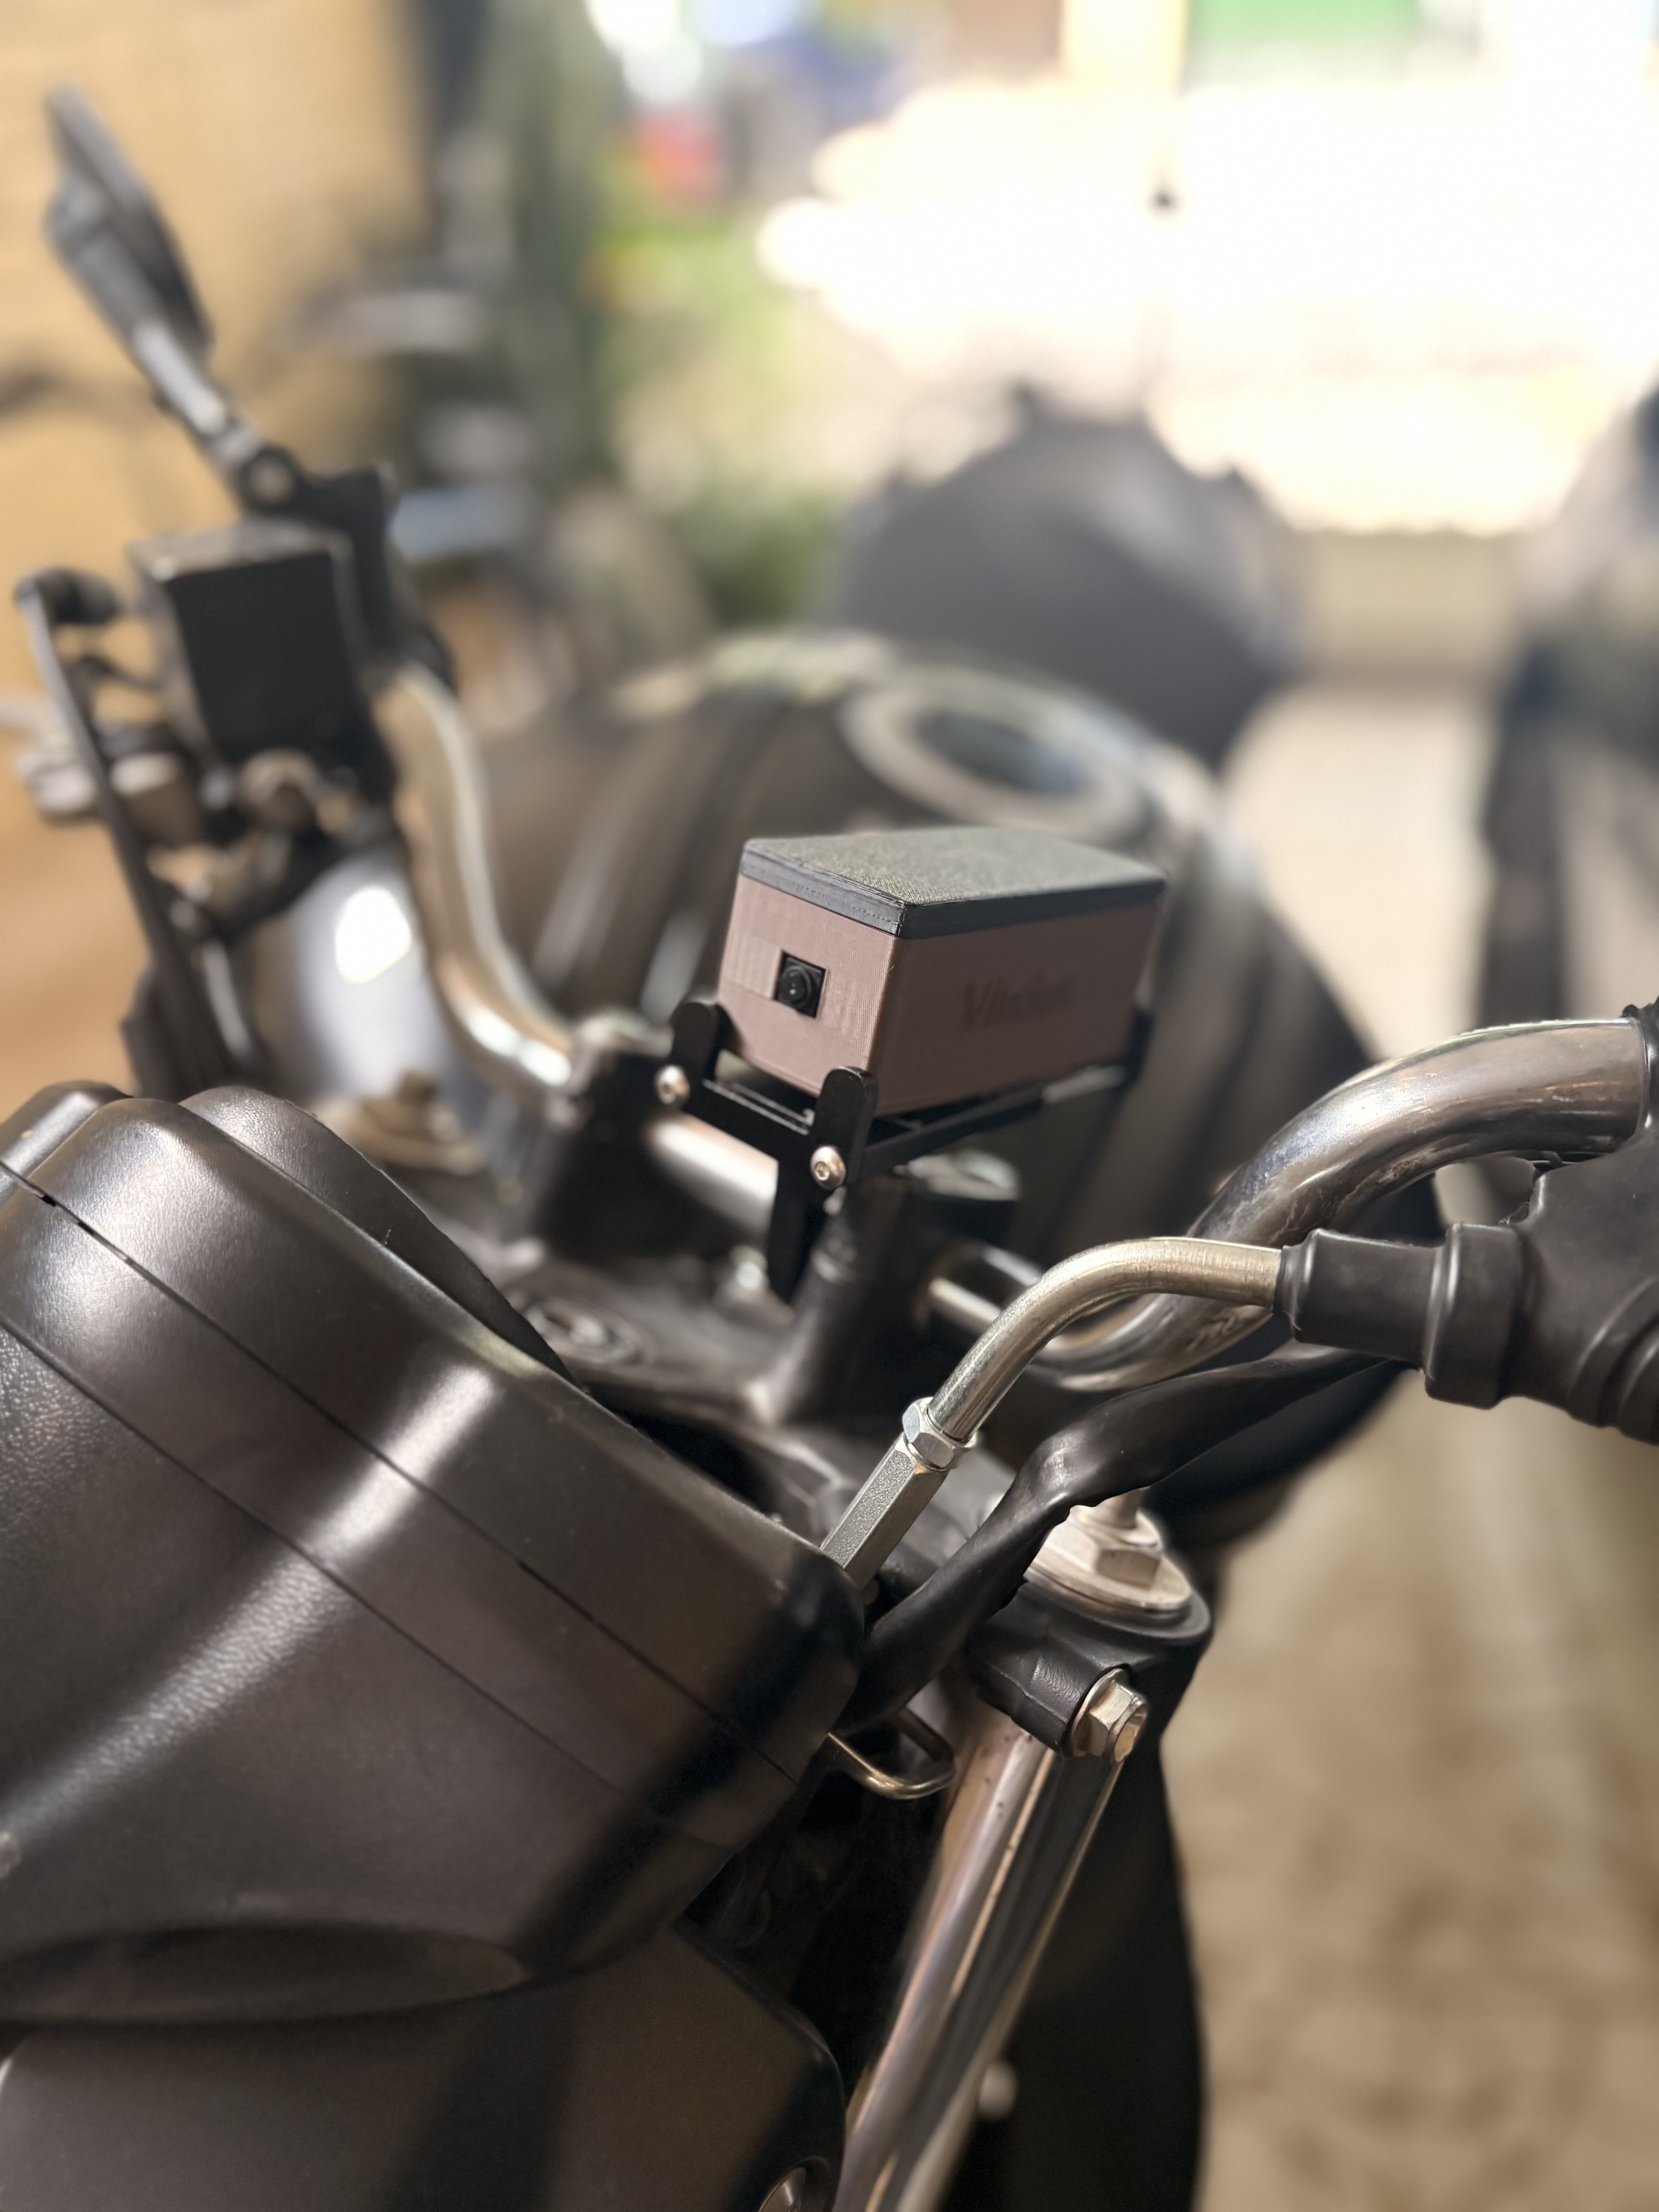
\includegraphics[width=0.7\textwidth]{prototipo-foto1.png}
\caption{Prot\'otipo do sistema desenvolvido - vis\~ao geral}
\label{fig:foto-prototipo}
\end{figure}

\begin{figure}[htb]
\centering
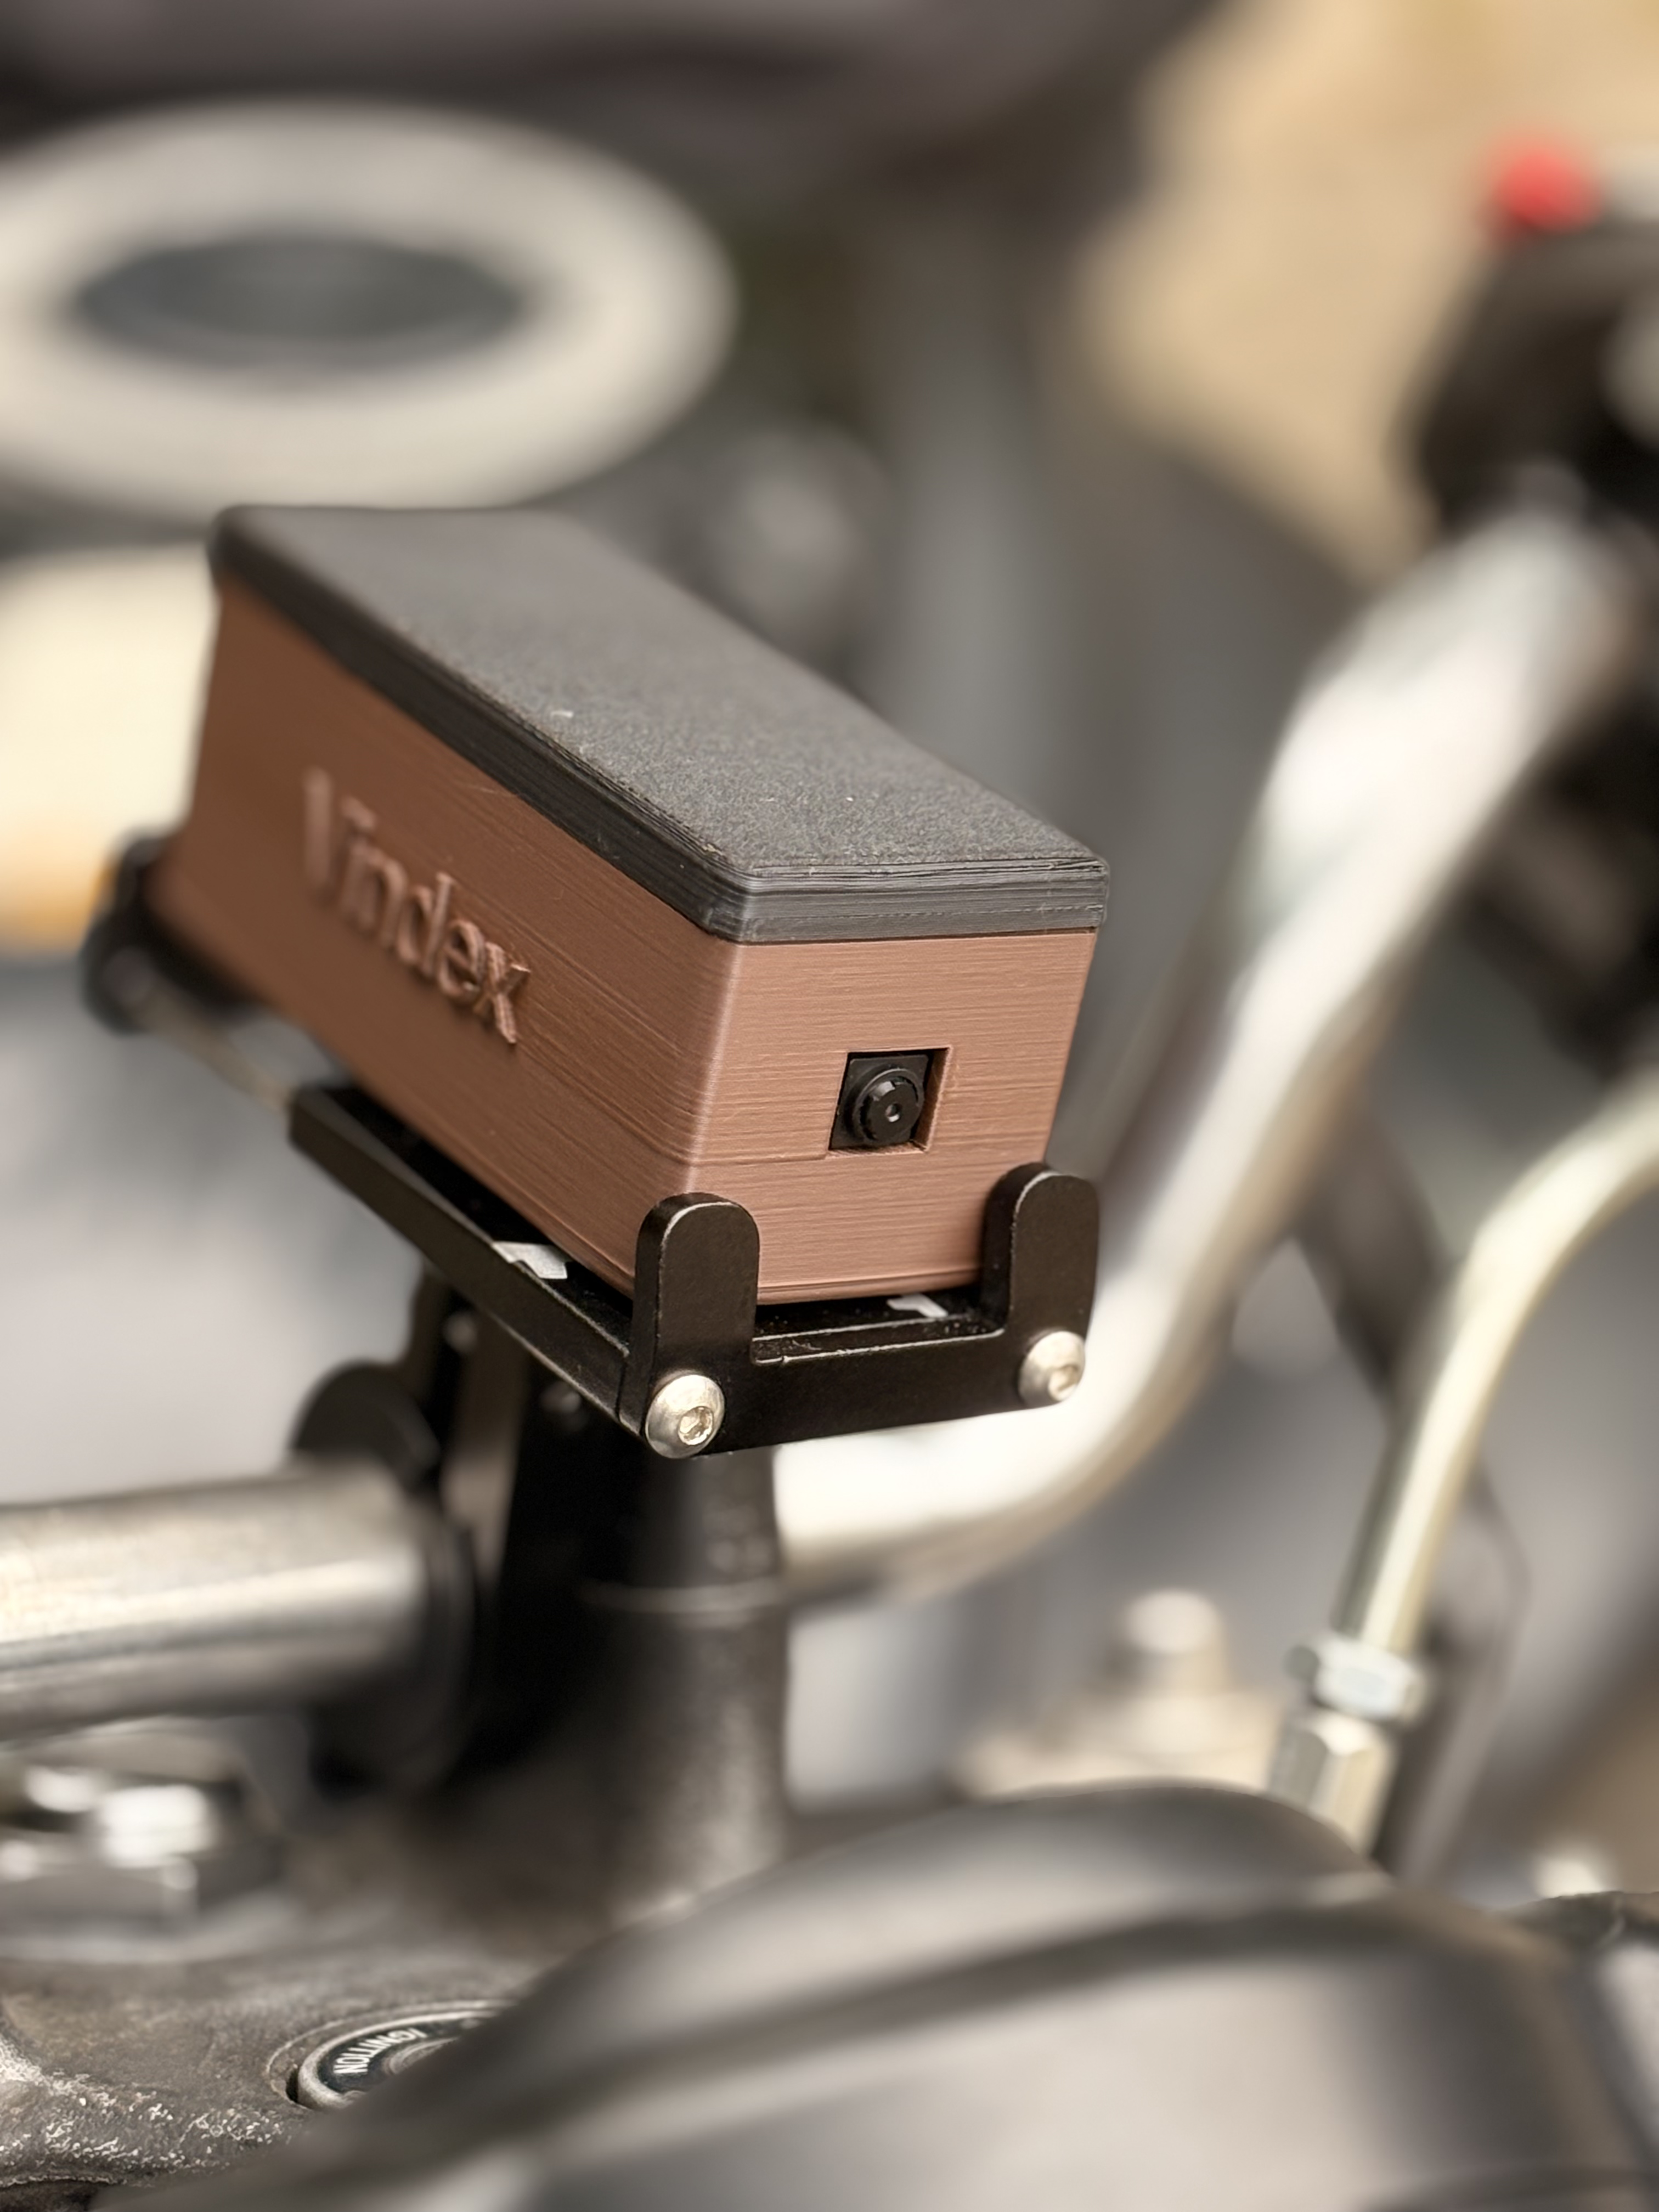
\includegraphics[width=0.7\textwidth]{prototipo-foto2.png}
\caption{Prot\'otipo do sistema desenvolvido - detalhes dos componentes}
\label{fig:foto-prototipo-detalhes}
\end{figure}

\chapter{Aplicativo iOS}
\label{ap:app}
Este ap\^endice apresenta capturas de tela do aplicativo m\'ovel Vindex desenvolvido para iOS, ilustrando as principais funcionalidades implementadas.

\begin{figure}[htb]
\centering
\includegraphics[width=0.4\textwidth]{app-tela-principal.png}
\caption{Interface de telemetria com resumo do per\'iodo: velocidades m\'axima e m\'edia, infra\c{c}\~oes e hist\'orico de viagens.}
\label{fig:app-tela1}
\end{figure}

\begin{figure}[htb]
\centering
\includegraphics[width=0.4\textwidth]{app-telemetria-grafico.png}
\caption{Tela de evid\^encia com detec\c{c}\~ao de placa (FBR2A23) via YOLO+OCR, mapa e detalhes do evento.}
\label{fig:app-tela2}
\end{figure}

\begin{figure}[htb]
\centering
\includegraphics[width=0.4\textwidth]{app-telemetria-historico.png}
\caption{Interface de telemetria com gr\'afico de velocidade e estat\'isticas de viagem (velocidade m\'axima 35,4 km/h).}
\label{fig:app-tela3}
\end{figure}

\begin{figure}[htb]
\centering
\includegraphics[width=0.4\textwidth]{app-evidencia-placa1.png}
\caption{Relat\'orio de viagem em PDF com mapa, an\'alise de seguran\c{c}a e perfil de velocidade.}
\label{fig:app-evidencia1}
\end{figure}

\begin{figure}[htb]
\centering
\includegraphics[width=0.4\textwidth]{app-evidencia-placa2.png}
\caption{Tela de evid\^encia com detec\c{c}\~ao de placa (HQW5678) via YOLO+OCR, mapa e detalhes do evento.}
\label{fig:app-evidencia2}
\end{figure}

\begin{figure}[htb]
\centering
\includegraphics[width=0.4\textwidth]{app-relatorio-viagem.png}
\caption{Relat\'orio de viagem em PDF com mapa de trajeto, an\'alise de seguran\c{c}a e perfil de velocidade.}
\label{fig:app-relatorio}
\end{figure}

\begin{figure}[htb]
\centering
\includegraphics[width=0.7\textwidth]{captura-1.png}
\caption{Captura de tela 1 do sistema.}
\label{fig:captura1}
\end{figure}

\begin{figure}[htb]
\centering
\includegraphics[width=0.7\textwidth]{captura-2.png}
\caption{Captura de tela 2 do sistema.}
\label{fig:captura2}
\end{figure}

\begin{figure}[htb]
\centering
\includegraphics[width=0.7\textwidth]{captura-3.png}
\caption{Captura de tela 3 do sistema.}
\label{fig:captura3}
\end{figure}

\begin{figure}[htb]
\centering
\includegraphics[width=0.7\textwidth]{captura-4.png}
\caption{Captura de tela 4 do sistema.}
\label{fig:captura4}
\end{figure}

\begin{figure}[htb]
\centering
\includegraphics[width=0.7\textwidth]{captura-5.png}
\caption{Captura de tela 5 do sistema.}
\label{fig:captura5}
\end{figure}

\begin{figure}[htb]
\centering
\includegraphics[width=0.7\textwidth]{foto-prototipo-fisica.png}
\caption{Fotografia do prot\'otipo f\'isico do sistema.}
\label{fig:foto-fisica}
\end{figure}

% Finaliza\c{c}\~ao do documento
\end{document}




